\documentclass[a4paper]{report}

\makeatletter
\renewcommand{\bibname}{References}
\renewenvironment{thebibliography}[1]
     {\chapter{\bibname}%
      \@mkboth{\MakeUppercase\bibname}{\MakeUppercase\bibname}%
      \list{\@biblabel{\@arabic\c@enumiv}}%
           {\settowidth\labelwidth{\@biblabel{#1}}%
            \leftmargin\labelwidth
            \advance\leftmargin\labelsep
            \@openbib@code
            \usecounter{enumiv}%
            \let\p@enumiv\@empty
            \renewcommand\theenumiv{\@arabic\c@enumiv}}%
      \sloppy
      \clubpenalty4000
      \@clubpenalty \clubpenalty
      \widowpenalty4000%
      \sfcode`\.\@m}
     {\def\@noitemerr
       {\@latex@warning{Empty `thebibliography' environment}}%
      \endlist}
\makeatother

\usepackage{geometry}
\usepackage[pdftex]{color,graphicx}
\usepackage{listings}
\usepackage{hyperref}
\usepackage{float}
\usepackage{listings}
\usepackage{paralist}
\usepackage{pdfpages}
\usepackage{enumitem}
\usepackage{algorithmic}
\usepackage{algorithm}
\usepackage{longtable}
\usepackage{titlepic}
\usepackage{pdfpages}
\setcounter{tocdepth}{2}
\hypersetup{colorlinks,citecolor=black,filecolor=black,linkcolor=black,urlcolor=black}
\graphicspath{{UIScreenshots/}{ClassDiagrams/}}

\title{\textbf{Bachelor project - Aegis Digital Voter List}}
\titlepic{
\includegraphics{AegisIcon.png}}
\date{\today}
\author{Nikolaj Aaes and Nicolai Skovvart.\\IT University of Copenhagen.\\Supervisor: Joseph Kiniry}
\begin{document}
\maketitle

\chapter*{Abstract}
Securing modern e-voting systems is a very challenging task. This paper describes an attempt to implement a secure digital system that could assist the current Danish voter card-to-ballot exchange protocol. The current approach is paper based and we have developed a digital solution with a strong focus on securing the data using encryption. The paper also discusses the different protocols for how election data is handled, transported and who interacts with it. We identify different kinds of attacks the system could be susceptible to, and present what kinds of countermeasures we have implemented to prevent any malicious behaviour from both outside and inside adversaries.

\tableofcontents

\chapter{Introduction}
Voting in Denmark is a paper based process prone to errors and it requires many resources. This paper describes the Aegis Digital Voter List system (Aegis DVL), designed to replace the current paper based approach of validating voters based on their voter cards with a software solution. The system handles sensitive data and needs to be resistant to malicious attacks and tampering. The paper discusses how network information is secured, how crashes are handled, how the data is distributed, and other relevant topics related to the system.

\section{Problem definition}
KMD developed a proprietary system used to generate and check voter cards. It provides little transparency and it can be hard to trust that it is secure, since the security can not be verified by the public. Is it possible to develop a transparent and secure alternative to KMD's solution? \\

The goal of this project is to design and develop an open source replacement for the proprietary, expensive Digital Voter List system developed and supported by KMD, used to generate and check voter cards in the 2011 national elections. The system will focus on data security and consistency. \\

Instead of reinventing the process, we have examined the KMD system and used some of the concepts. We are not building on top of the KMD system but rather investigating other ways to handle the same problems, both regarding design and implementation. A user of KMD's system should ideally be able to sit down and use the Aegis DVL system right away. 

\chapter{Scope}
The system is responsible for the exchange of voter cards to ballots, and not the actual votes. There is only one entry point in the form of the import of voter data and one exit point when the data is exported again. An election secretary is responsible for the election venue and election officials are responsible for handing out ballots to the eligible voters.
\begin{center}
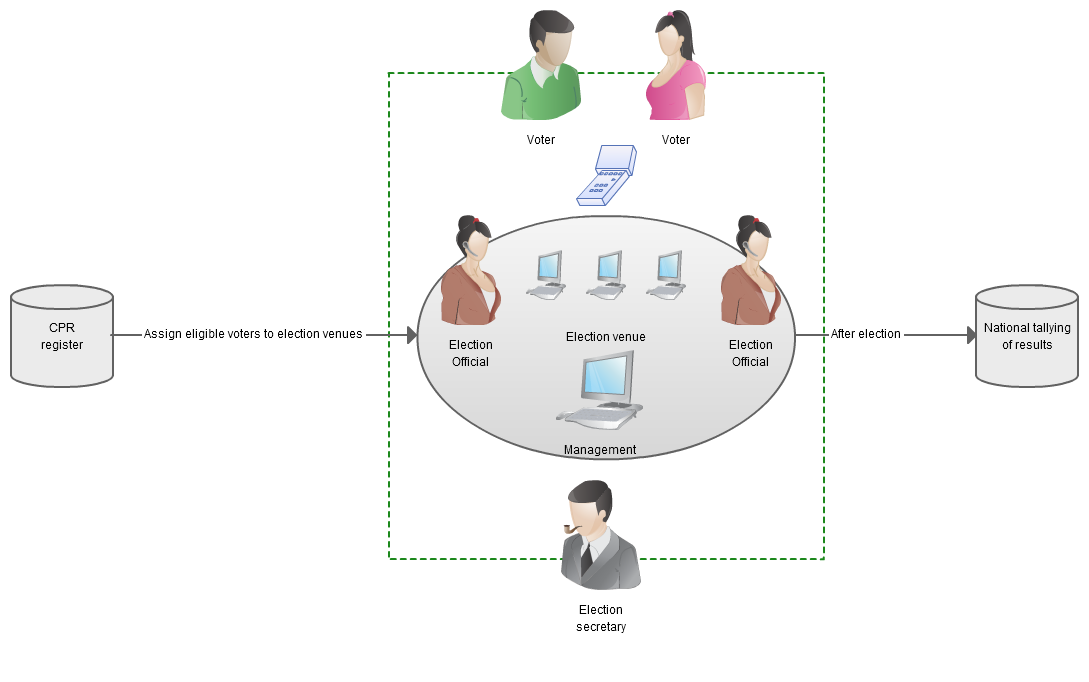
\includegraphics[width=\textwidth]{Domain.jpg}
\end{center}

This paper covers the following topics:
\begin{itemize}

\item A discussion of the design of the Aegis DVL system.

\item A discussion of what data is vulnerable and should be protected, and how the security is obtained.

\item A description of how synchronization and distribution of data is implemented in the Aegis DVL system and a brief discussion about the alternatives.

\item A description and discussion about the security measures taken to ensure that the voting data is protected and can not be tampered with. 

\item A user manual describing the common usage of the Aegis DVL system.

\item An overview of the testing strategy and the results.

\item Notes for any future developers of this, or a similar system. \\

\end{itemize}

Several other topics are not included in this paper:
\begin{itemize}

\item No usability analysis of the user interface has been performed. It is purely for demonstration purposes, and while containing the appropriate functionality, the aesthetics was not a priority.

\item This solution does not cover what happens before and after the election. This includes, but is not limited to, the partitioning of data, the printing and sending of voter cards, the storage of the machines, the collection of the data after the election has ended and the counting of votes.

\item This paper does not discuss the physical transportation of voter cards, machines, USB devices etc.\ in depth. While physical transportation is suggested several times one must consider the logistics and how the vehicle is guarded amongst other factors before implementing the solution in real life. 

\item The paper does not include an economical analysis concerning the Danish election protocols and how much money can be saved by using this solution instead of the existing one.

\item Neither an implementation nor a discussion of letter votes is included.
\end{itemize}

\chapter{Assumptions}
To reason about the systems and the work practices surrounding it, we have made certain assumptions:
\begin{itemize}
\item Both inside and outside adversaries will use any given opportunity to exploit the system. 
\item Adversaries have the required resources and time to carry out the attack of their choice.
\item The encryption algorithms can be trusted to encrypt and decrypt data in the manner explained in the documentation in a reliable fashion.
\item The algorithm chosen for generating keys can be trusted to generate matching key pairs in a reliable manner.
\item Danish CPR numbers are unique.
\item A single entity holds all CPR numbers and is able to partition them for the election venues.
\item A single entity will receive all the voter data from all the election venues after the election has ended.
\item The entity that prints voter cards and hands them out can be trusted.
\item No election venue will contain more than 25 machines.
\item It is unlikely for multiple machines to fail at once unless the system is being attacked.
\item Each election venue will handle at most 25.000 voters during the election.
\end{itemize}

\chapter{Requirements and Goals}
We wanted a system which was secure and user friendly. We wanted as little responsibility transferred to the election staff as possible which means that our program should be able to solve most problems without requiring attention from the user. With this in mind we devised the following requirements:
\\ \\ \noindent \bf Primary requirements: \rm
\begin{itemize}
\item Features
\begin{itemize}
\item Must be able to register when a voting ballot has been handed out, and prevent it from happening multiple times.
\item Must be able to confirm whether a voter is eligible to be handed a ballot based on a CPR number and a voter number.
\item Must support a management machine with elevated privileges.
\item Must have a graphical user interface.
\item At least the management machine, must be able to display relevant data about the election and status of the stations.
\end{itemize}
\item Code requirements
\begin{itemize}
\item Unit tests must cover at least
\begin{itemize}
\item 90\% of the station/manager-code.
\item 90\% of the code of the database-layer.
\item 90\% of the code of the crypto-layer.
\item 90\% of the core data-types.
\end{itemize}
\item Other tests must include
\begin{itemize}
\item The scanner.
\item The printer.
\item The user interface.
\item The communication-layer.
\end{itemize}
\item Must use code contracts.
\item Must be thoroughly documented.
\end{itemize}
\item The system
\begin{itemize}
\item Must be able to recover from common network errors.
\item Must be able to track if a voter card has been printed for a person.
\item Must allow a voter to use any of the stations at the election place.
\item Must allow extraction of the full data set on at least the management machine, at any given time during the election.
\item Must be able to generate voter cards.
\item Must be able to scan voter cards.
\item Requires at least four machines to operate, of which, one is a management machine.
\item Requires that adding or removing a station must be approved by at least the management machine.
\end{itemize}
\end{itemize}

\noindent \bf Secondary goals (optional): \rm
\begin{itemize}
\item It should be faster to use the system than using the current paper-based model.
\item The system should be able to generate a list of all the voters of the election place and whether they have voted or not and print it.
\item The graphical user interface should be easy to learn and use.
\item The system should support letter votes.
\item Use a data flow analysis tool to reason about correctness of the data flow in the system.
\item Use an analysis tool to reason about the cryptographic protocol used.	
\end{itemize}

\noindent By implementing a solution that fulfills these goals we made sure we had a well tested, documented and robust system that enabled the current work practices to be carried out in a secure manner while still being conducted inside the boundaries of the law. \\

Ideally the unit tests should cover 100\% of the code, but as some code is hard or impractical to test, like the user-interaction and some netcode, we lowered the requirements to 90\% code coverage to provide some leeway. 

\chapter{Design and Architecture}
\section{Overview}
The system we have designed consists of one manager machine and at least three station machines with the ability to add more. Each of the machines will have an attached barcode scanner that enables voters to scan their voter cards. A voter can type his CPR number into the system and scan his voter card which makes the system check if he is eligible to receive a ballot. If he is, an election official should hand him a ballot. \\

The system needs to be distributed because the data needs to be shared between the machines. For a discussion on how this is achieved, see section \ref{sec:data} Data. The sharing itself is done through the local network and this could potentially be a security concern. We require that users of the system makes sure they are connected to a closed, wired network during the entire election. This is discussed further in section \ref{sec:security} Security.\\

Since the data the system is handling is personal sensitive data, encryption of the data is essential. We strove to have the data encrypted at all times to make sure that both outside and inside attacks would be as hard as possible. This applies to the databases containing the voter data and the logs as well as the data being transmitted over the network. \\

To use the system one must have an encrypted data set of the voters that are eligible to vote at the election venue and the encrypted key used. This data is loaded into the system on the manager machine and when it connects to a station it is distributed to that station. The manager machine generates a master password which is used to start an election, end an election, mark a voter as having received a ballot with his CPR number only, and access the log database.\\

When the manager machine has connected to the desired stations, it can start the election. When this is done all the machines switch to a screen where it is possible to enter a voter number and a CPR number. It is also possible for the manager machine to remove or add additional stations on this screen. When a voter enters his voter number and CPR number and pushes the "F\ae rdig" button, the system checks whether he is eligible for a ballot or not. If a voter has lost his voter card, the election secretary can mark a voter as having received a ballot, using just his CPR number and the election venue master password. \\

When the election ends all the stations close their application and the manager machine can export the data to a file location. The exported data is still encrypted and can only be decrypted by the holder of the initial decryption key, that was generated with the voter data encryption key. \\

As a rule of thumb, the system was designed to shut down the election if the suspicion of an attack is raised. Since no guarantees can be given about a data set that was potentially a victim of an attack, the risk is too high to continue the election. If the manager machine becomes unreachable, an election for a new manager will start and an active station will be promoted to be the new manager when it ends. This promotion can also be done through the manager's user interface. If a station becomes unreachable it will be removed from the list of active machines the other machines know.

\section{Design}
Choosing the right security mechanisms was a major part of our design decisions and we approached this using the twelve principles presented in Applied information security: A hands-on approach \cite{basin} which are discussed in section \ref{sec:security} Security. \\

We have used the BON design language \cite{bon} in our design process to get a complete overview of our application before producing any code. We used code contracts \cite{codec} to make sure the application behaved as expected as dictated by the Design by Contract principle \cite{dbc}. \\

To improve the modularity of the application we provided interfaces for all the major classes except for Station. This makes for easy replacement of parts of the program which might become needed later on. We used the Mediator pattern \cite{medi} when we implemented the user interface since we wanted it to be easily replaceable with any user interface. The only requirement would be to implement the IDvlUi interface to make sure the back-end of the system could communicate with the user interface. \\

As for the messages sent from machine to machine we used the Command pattern \cite{cmdp} which provided us with an easy way to encapsulate data and instruct the target machine what to do with it. 

\section{The main classes}
To provide an overview of the classes in the application we have created a class diagram which can be found in Appendix \ref{sec:classd} Class Diagrams, along with descriptions of the major classes in the system:

\subsection{Station}
The Station class is the large back-end class that contains the core functionality for the station and manager machines. While a station machine and a manager machine have semantically different meanings, in the code, the Station class contains functionality for both, since a manager machine is merely a station machine with elevated rights and responsibilities. As such we have compiled a list of functionality the Station class contains and whether it is used by the manager machine or a station machine:

\begin{itemize}
\item Station
\begin{itemize}
\item Start election for new manager.
\item Request a ballot.
\end{itemize}


\item Manager
\begin{itemize}
\item Add/remove stations.
\item Transfer manager-status to station.
\item Check status of stations.
\item Start election.
\item End election.
\item Manually mark selected voter as being handed a ballot (in case they lost their voter card).
\end{itemize}
\end{itemize}

\subsection{Crypto}
The Crypto class is responsible for all encryption and decryption related actions. It can encrypt and decrypt with both symmetric keys and asymmetric key pairs. It is also used to generate the master password and the required key pairs. If the encryption and decryption algorithms need to change, a new Crypto class can be constructed and used as long as it implements ICrypto.

\subsection{Communicator}
The Communicator class is responsible for the network communication between machines. It both sends and listens for commands, and executes each command as it is received. If the network protocol needs to change, a new Communicator class can be constructed and used as long as it implements ICommunicator.

\subsection{SqLiteDatabase}
The SqLiteDatabase class facilitates all queries to the database. This system uses an SQLite database, but it can easily be changed and the alternatives are discussed in section \ref{sec:dbms} Database management system (DBMS). If the DBMS needs to be changed or one wants to change to a different kind of data storage, a new database class can be constructed and used as long as it implements IDatabase.

\subsection{Logger}
The Logger class is responsible for all log entries and exporting the log. Whenever an important event in the system occurs, the Logger class sees to that it is logged in the right place with the right encryption. No logging framework is used by our logging class, but if one wanted to add a framework or change the way the logs are stored, a new Logger class can be constructed and used as long as it implements ILogger.

\subsection{UiHandler}
The UiHandler is responsible for all user interface related communication. Every time the user interface wants to use methods from the station and the other way around, it results in a call to the UiHandler. If the user interface needs to be replaced a new UiHandler class can be constructed and used as long as it implements IDvlUi.

\section{Generating voter cards}
One of the requirements for the system was the generation and printing of voter cards. To accommodate this we have added a PDFGenerator project written by K\aa re Sylow Pedersen as a part of the Digital Voter Registration System \cite{dvrs}. The code can generate voter cards and lists of voters and requires code contracts to be installed. This is not part of the user interface, because generating and printing voter cards takes place before the election starts, and will not be printed at the election venues. Every time a voter card is printed, it should be saved in an appropriate database. There is no reason for this data to be distributed to the election venues since it is not used in the system, but the entity printing the voter cards might have a use for it. \\

It is recommended to use a scanner with our current user interface since the generated voter cards have barcodes associated with their voter number. We tested the system with a Symbol HotShot LS2106 barcode scanner which essentially fires keyboard events when it scans. As long as the correct text box has focus the scanning works as intended. This scanner was produced in may 2000 and uses a PS/2 keyboard input. 

\section{Contract coverage}
We have used code contracts in our system to ensure that our code will always function as long as the contracts are respected. It also makes debugging easier as a failed precondition will stop execution immediately instead of passing potentially bad parameters to other methods. The use of preconditions also allow us to ignore a lot of exception-throwing code as errors can be made impossible as long as preconditions are abided by. The contracts cover the following of our code.

\noindent 
\begin{table}[ht]
\centering
\begin{tabular}{|c|c|}
\multicolumn{2}{c}{Contract coverage results}\\\hline
\textbf{Domain} & \textbf{Count}\\\hline
Total amount of methods & 158 \\
Methods covered by contracts & 93 \\
Lines of contract-code & 189\\
Lines of non-trivial contract-code & 39\\
Class-invariants & 9\\\hline
\end{tabular} 
\end{table}\\ 

It is worth noting that a lot of the methods that are not covered are auto-property getters that are unable to guarantee anything. The majority of the contracts are trivial requires-not-null checks or ensures-not-null checks. Some of the more interesting contracts requires that stations are (or are not) currently listening to TCP requests, or requires that the machine is currently the manager.

\chapter{Data}
\label{sec:data}
This system handles a lot of data transactions and most of this data is personal and sensitive. People do not want everyone knowing their CPR numbers and whether they have voted or not. Before an election can start, each election venue needs a list of voters that should be able to hand in their voter cards in exchange for a ballot and vote at their specific location. Initially all this information is stored in a single location and needs to be partitioned for each election venue. This partitioning will most likely be based on the addresses of the voters, but in this paper we do not discuss how this partitioning should be conducted. 

After the partitioning, the different fragments must be transported to the election venues. This can happen in a few different ways:

\begin{itemize}
\item Use the Internet to transmit the data.
\item Use a messenger service to transport it via a portable medium (USB device, CD etc.).
\item Use your own messenger to transport it via a portable medium.
\end{itemize}

We strongly recommend the "Use your own messenger to transport it via a portable medium"-approach to reduce the attack surface for adversaries and to gain more control of the transportation. The transportation should preferably be guarded, but the financial costs of this might exceed the benefits.

\section{Receiving and distributing data}
\label{sec:RaDdata}
When the partitioned data arrives at the election venue it needs to be distributed to all the machines in the election. To make it easier for the person who needs to set up the machines at the election venue it is assumed that there is a single point in the closed network that receives the collection of eligible voters. This makes for a few possible solutions for receiving the data:

\begin{itemize}
\item A manager machine receives the data and distribute it to the other machines.
\item A station machine receives the data and distribute it to the other machines.
\item Either a manager- or a station machine can receive the data and distribute it.
\end{itemize}

Alternatively the data could be distributed manually via a portable medium, but this is unnecessarily cumbersome. We have chosen that the manager machine receives the data and distributes it. Since the manager is the machine managing the stations, it makes sense to have this machine join the task of receiving and distributing data with the task of connecting to all the stations. \\

The data can be distributed among the machines in several different ways each with its own advantages and disadvantages.

\begin{description}[style=nextline]
\item [Every machine has the full data set all the time.] This solution has the advantage of being the most robust, because the data is not lost if a machine crashes, since all the other machines will have a full backup of all the data. The disadvantages are that the network traffic required to makes sure that the data set is up to date on all the machines is quite high compared to the other solutions. Also, if an adversary was to gain access to any machine he would have access to the full data set which leaves him with a larger attack surface.

\item [Every station has a partition of the data set and the management machine has either no data set, the full data set or a backup partition based on some criteria.] This solution uses less network traffic since it only needs to synchronize the station with the relevant part of the data. Also this solution leaves less options for adversaries to gain access to the full data set since each machine only has a partition. The disadvantages is that the solution is very prone to adversaries that seek to destroy the election. If even a single machine crashes, its entire data set is lost. This can be circumvented by having a backup of the full data set stored on the manager machine which will increase network traffic, but provide a full data set which increases the attack surface.

\item [Every station has two or more partitions of the data set, one partition belonging to the station itself and one or more backups of the other stations. The management machine can have data sets like in the second solution.] This solution improves on the previous solution by having a more robust design. In this solution a machine can crash without the loss of data since a backup is always kept on another machine. This increases the network traffic, but leaves the full data set partitioned making it harder for adversaries to obtain it.

\item [The management machine has the full data set and the stations contain no data.] This solution focuses on storing as little data as possible on the stations. Since the stations are the most vulnerable machines, as they are handled by the voters, they contain no data at all. This is somewhat network traffic intensive for the manager, compared to the other solutions, since every update is sent to the manager who then updates the database. It is also quite a dangerous solution since the manager machine becomes a single point of failure. If it crashes the entire election data is lost. Against adversaries this is both advantageous and disadvantageous since the stations have no data that can be obtained, but the manager machine has the full data set. If the adversary is aware that the data is located on the manager machine only, he has no need to attack the stations.  

\item [A separate database is located in the election venue and the management machine takes the role as a proxy to facilitate communication between stations and the database.] This solution is quite similar to the previous solution, but the data is now moved to a separate machine. This is an advantage because the manager machine facilitates other features and is therefore more prone to errors and attacks than a separate machine which no one interacts with. The disadvantage is an increase in network traffic since the manager now has to forward all requests and answers from the separate database. This solution still has a single point of failure which, from a distributed systems viewpoint, is a serious disadvantage.

\end{description}

We chose to use the first solution for its robustness. We realized that we needed to focus on making each machine as secure as possible since they all contain the full data set, but being able to recover from the crash of any machine is a desirable property. While this solution is traffic intensive, we do not sacrifice any robustness and in a real world scenario each election place has at most 25 machines in total, which makes the traffic almost unnoticeable. The system might not scale in an ideal manner, but the security aspect takes priority over performance.

\chapter{Synchronization and Broadcasting}
Since we chose a robust solution where every machine has the entire data set at all times, we need a way to synchronize all the machines to make sure that all the data sets are up to date if any of them should crash. There are several ways this can be done:

\begin{itemize}
\item  \textbf{Request synchronize}
- A station requests the manager machine to synchronize all the other machines with a certain update set.
\item \textbf{Broadcast}
- A station broadcasts an update set to all other machines.
\item \textbf{Epidemic}
- A station utilizes an epidemic protocol to update all other machines.
\end{itemize}

\noindent This synchronization can be initialized at different times during the election:
\begin{itemize}

\item \textbf{On action}
- After every action (a voter scans a voter card) on a station, a synchronization is initialized.
\item \textbf{Interval}
- At a certain time interval a system wide synchronization is initialized.
\item \textbf{Key-points}
- At certain key points (eg.\ after 100 voter cards have been scanned) a system wide synchronization is initialized.
\end{itemize}

We have chosen a combination of "Request Synchronize" and "On action". By using the manager as a mediator when an update is to be propagated to the machines in the network, we obtain a simpler communication channel which is easier to reason about and test. We chose "On action" updates because we want the updates to happen every time a voter has been handed a ballot, to ensure, that if a machine crashes its data is not lost. We realize that this generates a large amount of messages, but it satisfies our condition, that every machine must have the full data set all the time as described in section \ref{sec:RaDdata} Receiving and distributing data. \\

\noindent Once again there are several ways we can do this:
\begin{description}

\item [Our own algorithm] - with this approach an update message is sent from a station to the manager every time a voter requests a ballot. The manager checks its own database and if the voter is eligible for a ballot, it sends a message to every station other than the initial one telling them to update their database. Lastly the manager sends an update (and confirmation) to the initial station which then hands out the ballot. If the initial station becomes unavailable (i.e.\ crashes) before it can receive a confirmation, the manager sends out a revoke command to every other machine telling them that the ballot has not been handed out and that their database should reflect that. It is important that the manager sends the update messages at the same time, because the system can not handle a situation where the manager crashes halfway through updating the stations. That leaves some stations with one ballot status and some with another and no manager to confirm which one is correct. If a station is unreachable when an update message is sent, it is removed from the manager's and the active stations' list of connected stations.

\item [The ChandyLamport algorithm (Snapshot algorithm)] \cite{lynch} \cite{chandy} - with this approach an observer process initiates the algorithm to gather a global snapshot of the system. If we were to use this algorithm it would have to be modified since we wanted updates to be communicated to other machines when a ballot has been handed out, and this algorithm only updates the initiator. The most significant problem however, is the fact that the entire state of each machine would be sent over the network. This could potentially be thousands of entries which is unnecessary for our purposes.

\item [NSync] \cite{nsync} - NSync would be a good choice if we wanted to have several updates at a time on each machine. It works by sending metadata on what changes needs to be made, resolves conflicts and afterwards sends the necessary data for the changes to happen. It would not be fit for our purpose since we want to send one update at a time and because that conflicts in the data sets, is a reason to suspect that a machine has been compromised in our system.

\end{description}

To provide better insight into how our algorithm is implemented, the following pseudo code is supplied:
\begin{algorithm} [H]
\caption{Our synchronization algorithm - Station side}
\begin{algorithmic}[1]
\STATE $VoterNumber \leftarrow$ Scanned VoterNumber
\STATE $CPR \leftarrow$ Typed CPR
\STATE $Check \leftarrow CheckOwnDatabase(VoterNumber, CPR)$ \COMMENT {returns false if the voter does not exist or has already received a ballot}
\IF{$!Check$} 
\STATE $InformVoter()$ \COMMENT{inform the voter that he does not exist or has already received a ballot}
\ELSE
\STATE $Manager.RequestBallot(VoterNumber, CPR)$ \COMMENT {sends a command to the manager with the request}
\ENDIF 
\end{algorithmic}
\end{algorithm}

\begin{algorithm} [H]
\caption{Our synchronization algorithm - Manager side (RequestBallot)}
\begin{algorithmic}[1]
\STATE $VoterNumber \leftarrow$ Scanned Voter Number
\STATE $CPR \leftarrow$ Typed CPR
\STATE $Check \leftarrow CheckOwnDatabase(VoterNumber, CPR)$ \COMMENT {returns false if the voter does not exist or has already received a ballot}
\STATE $UpdateOtherStations(VoterNumber, CPR)$
\IF{$IsActive$(Sender)}
\IF{$Check$}
\STATE UpdateSender(true) \COMMENT {sends a command to the sender telling it to update its database and tell the voter he can receive a ballot}
\ELSE
\STATE UpdateSender(false) \COMMENT {sends a command to the sender telling it not to update its database and tell the voter he can not receive a ballot}
\ENDIF
\ELSE
\STATE $RevokeBallot(VoterNumber CPR)$ \COMMENT{revokes the ballot status on all the other stations}
\ENDIF
\end{algorithmic}
\end{algorithm}

To ensure that our algorithm works as expected, we used the model checking tool UPPAAL \cite{uppaal}. By using this tool we were able to verify that our synchronization algorithm updates all the machines when a ballot is handed out, and that each voter can only be handed one ballot. Screenshots from the verification can be found in appendix \ref{sec:uppaal} UPPAAL. \\

We considered the fact that if an election venue has a large amount of stations, the manager might get a message implosion where too many messages are to be handled at the same time. Implementing a queue system on the manager side of the communication layer should be sufficient to handle the inbound messages. If this was a greater concern Schooler's suppression algorithm \cite{schooler} would be a viable way to avoid this problem.

\section{Database management system}
\label{sec:dbms}
To manage the data on each machine, our system uses a database management system (DBMS). We have made it easy to exchange this DBMS with another one by defining an interface for the database layer. If one were to exchange the current DBMS the properties of the new DBMS should be considered. Some desirable properties are:

\begin{itemize}
\item ACID (atomicity, consistency, isolation, durability)  transactions either through locking or multi-versioning.
\item Security layer for encryption.
\item Scalability.
\item Logging framework.
\end{itemize}

\noindent One might consider a DBMS with a distributed protocol to handle consistency over a network, but we have chosen one without it to get a greater degree of control on how the data in synchronized between the machines. If a DBMS with a distributed protocol is chosen, it needs to have eventual consistency within a time frame (depending on the amount of stations) to make sure the election machines are consistent between every ballot handed out. We suggest an open source system for several reasons; an open source DBMS project could be forked to fulfill possible future requirements, it would be possible to have a peer review of the crypto layer and other security aspects, and it would also be consistent with our own open source project. There is nothing preventing the use of a proprietary system, though. 

We have provided a list of some of the database management systems that could be usable and what properties they fulfill. 

\noindent \begin{tabular}{|c|ccccc|}
\multicolumn{6}{c}{Database Management Systems}\\\hline
Name & Developer & Open source & Crypto layer & ACID & Maintained\\\hline
REDIS\cite{redis} & Salvatore San Fillippo & Yes & No & No & Yes \\
MongoDB\cite{mongo} & 10gen& Yes & No & No & Yes \\
CouchDB\cite{couch} & Apache Software Foundation & Yes & No & Yes & Yes\\
MySQL\cite{mysqlcrypt} & MySQL & Yes & Yes & Yes & Yes\\
PostgreSQL\cite{postgre} & PostgreSQL & Yes & Yes & Yes & Yes\\
SQLite\cite{sqliteee} & SQLite & Yes & Yes & Yes & Yes\\ 
DBMS\_crypto\cite{dbmscrypto} & Oracle & No & Yes & Yes & Yes\\
MSSQL\cite{hsueh} & Microsoft & No & Yes & Yes & Yes\\
Sybase ASE\cite{sybase} & Sybase & No & Yes & Yes & Yes\\
DB2\cite{db2} & IBM & No & Yes & Yes & Yes \\
Firebird\cite{firebird} & Firebird & Yes & No & Yes & Yes\\
Microsoft Access\cite{access} & Microsoft & No & Yes & No & Yes\\\hline
\end{tabular} \\ \\

We have decided to implement the database using SQLite \cite{sqlite}. SQLite is a "\textit{software library that implements a self-contained, serverless, zero-configuration, transactional SQL database engine}"\cite{sqlite}. We decided to use this DBMS as it fulfills all the desired properties, it was fast to install and implement, and it did not require the use of external systems. To interact with the database, we use the ADO.NET Entity Framework \cite{adonet}.

\chapter{Security}
\label{sec:security}
Security is an essential part of every system in the domain of elections. Making sure that the election can not be tampered with, is of the highest priority because the information could potentially have consequences for a lot of people. We approached this using the twelve principles presented in Applied information security: A hands-on approach \cite{basin}:
\begin{description}[style=nextline]
\item [1. Simplicity - simpler security mechanisms are easier to understand and maintain.]
We designed a system that introduces as few new concepts as possible, so users of the current paper-based solution should find the application easy to use.

\item [2. Open design - a system should not depend on the secrecy of its protection mechanisms.]
Our system is open source and everyone can examine the code. If the security was dependant on the secrecy of the mechanisms it would effectively have no security at all. We have designed mechanisms that depend on the secrecy of generated keys and not knowledge of the mechanisms themselves.

\item [3. Compartmentalization - Organize resources into isolated groups of similar needs.]
We have divided the code into classes corresponding to their responsibilities. We have provided interfaces for some of the more interesting classes which makes it easy to replace and maintain them.

\item [4. Minimum exposure - minimize the attack surface the system presents to the adversary.]
By providing the minimum amount of opportunities for manual input from anyone and operating in a closed network we strove to minimize the attack surface as much as possible.

\item [5. Least privilege - any component of a system should operate using the least set of privileges necessary to complete its job.]
We keep all data encrypted during the entire election to prevent anyone, even an insider, from tampering with the data. Decrypted data is never stored and as soon as new data enters the database it gets encrypted. By using a master password we ensure that only the appropriate members of the election staff has the privileges to perform certain actions such as marking a voter using only their CPR number.

\item [6. Minimum trust and maximum trustworthiness.]
We choose to minimize the trust between the different machines. Every message sent over the network is validated and if the message is not accepted, the election will switch to a paper based approach since the sender is regarded as compromised. 

\item [7. Secure fail-safe defaults - the system should start and return to a secure state in the event of a failure.]
We use several detection mechanisms to catch failures and handle them. See section \ref{sec:detection} Detection and recovery.

\item [8. Complete mediation - access to any object must be monitored and controlled.]
By using code contracts and rigid logging we monitor all access to the data. To control access to the system we only accept incoming net traffic in a certain format and to control the access to the data we use our database layer which can only be accessed through the application. 

\item [9. No single point of failure - build redundant security mechanisms whenever feasible.]
We do not want any machine to be a single point of failure, and by having all the data distributed to all the machines we can handle the crash of any machine. 
If the manager machine should crash the stations can elect a new manager and continue with the election.

\item [10. Traceability - log security-relevant system events.]
We store logs locally on each machine encrypted with the master password ensuring that the log is accessible even after a system crash.

\item [11. Generating secrets - maximise the entropy of secrets.]
All of our generated secrets are created using Bouncy Castle's \cite{bouncy} SecureRandom class. Randomly generated numbers are generally too predictable and thus insecure, so a strong source of randomness is needed. We trust that the implementation by Bouncy Castle is sufficiently secure.

\item [12. Usability - design usable security mechanisms.]
The system uses several different mechanisms and we have automated as many as possible. We require very little of the users, and the tasks the users have to perform are trivial.

\end{description}

By following these principles we got some desirable properties for our system. The next thing to consider was what kind of attacks our system could be a victim of. For this we used the STRIDE \cite{meier} threat categories and the corresponding countermeasures:

\begin{description}
\item [Spoofing]
- We use strong authentication and store all the data in an encrypted fashion.
\item [Tampering]
- We use a secure communication protocol and hybrid ciphers. 
\item [Repudiation]
- We use logs and digital signatures to ensure this.
\item [Information disclosure]
- We use strong encryption algorithms. 
\item [Denial of service]
- We make sure that the machines are on a closed network with no access to the Internet.
\item [Elevation of privilege]
- We follow the Least Privilege principle.
\end{description}

The system must be connected to a closed network during the election, only potentially connecting to the outside to import partitioned voter data prior to the election or upload exported voter data afterwards. To ensure that the network is actually closed the connection must always be wired and not wireless. The unused port in the switch/router must be obstructed thus preventing adversaries from plugging their own machines in and accessing the network. Ideally the switch/router is in the same location as the manager machine to make monitoring both of them at the same time convenient.\\

To avoid that voters or election staff accidentally close the application during the election, we have disabled the red x in the upper right corner of the application. As an additional security layer we would have liked to implement the application in such a way that it would run as a service and require administrator rights to close it to further increase the security. \\

The master password and the decryption key to the data set are each entrusted to a single entity, which means that the two entities in question must be trusted. Ideally each of these keys would be split into several fragments and each fragment given to a different entity, preferably with different stakes in the election. Only by using all the fragments at the same time would the key be usable. This would place the trust on several entities instead of a single one and make it harder for adversaries to acquire the combined key. This is not a practical solution for the master password since you would have several entities typing on the same machine each time a voter has lost his voter card, which would be cumbersome. But for the decryption key, this would be a thing to consider when decrypting the voter data. 

\section{Attack model}
To identify and assess threats to the system we created attack trees \cite{schneier} using the notation described by Moore et.al. \cite{moore} with added notation for reusing attack patterns inside the attack trees to provide smaller and clearer attack trees. The full attack trees can be found in appendix \ref{sec:atrees} Attack Trees, where the additional notation is also described. Constructing attack trees is a method to identify different kinds of attacks against a system, consider the likelihood and resources required of each attack and manage the risks. The weakness of this approach is that it relies on the creator to consider all the different kinds of attacks and predict the correct probabilities and resources. The detail and depth of the attack tree is also decided by the creator and important information might be omitted. Since this is a paper primarily concerning software, we have chosen to focus our attacks on how one could destroy or tamper with an election via our software. By identifying the possibilities of potential adversaries we produced countermeasures and implemented a more secure solution. \\

The outcome of constructing attacks trees was knowledge of where to focus our efforts when designing the security of our software and we arrived at several conclusions:

\begin{itemize}
\item The portable medium used to transport the data from the partitioning venue to the election venue should have a protection mechanism to prevent tampering with the data prior to and after the election. This could potentially be solved by having the data obfuscated or signed, and the deobfuscation password only being exchanged securely when the data is at the election venue.
\item Access to the machines used for the election must be very limited before and after the election. It should be impossible for unauthorized personnel to gain physical access to the machines prior to and after the election.
\item The process of identifying voters that lost their voter cards must be very thorough before handing them a ballot to prevent impersonation.
\item Being connected to the Internet can be a huge threat and should be avoided as much as possible.
\item Data should be checked every time it travels from one machine to another to prevent using corrupt or invalid data.
\item The hardware facilitating the network should be under observation during the election to prevent unintended machines from connecting to the network.
\item Connecting to the network of machines running the software should require authentication to make it harder for adversaries to gain access to the network.
\item The less decryption that takes place during the election the better. Ideally each machine should only be able to see the data it needs and nothing more thus following the Least Privilege Principle \cite{basin}.
\item The election personnel should consist of trusted individuals. Even though the software will protect against insider attacks, they are still one of the greatest potential threats.
\item The generation of the keys used to encrypt the initial data set and decrypt the final data set should be conducted in a safe location since the acquisition of these could compromise the entire election.
\item The machines used in the election should be dedicated only for the election. This should prevent the machines from being compromised prior to the election. Alternatively the machines could be reset to factory standards instead of being dedicated. 
\end{itemize}

In the attack trees the attack pattern "Manipulate persons" is used repeatedly indicating that this is a weak point in the security structure. When in a real life environment, it is therefore important to make sure that the election staff is well protected and not likely to receive bribes. When the "Manipulate persons" attack pattern is used, it is often to gain access to a certain encryption or decryption key, or to the election venue and hardware. This is something that is available to the election staff as well, and if the adversary knew an insider, or was an insider himself, the "Manipulate persons" attack pattern would not be a necessary action for the attack to succeed. It is important to notice that the attack trees are devised from an outside adversary's point of view and many other obstacles would be removed as well if the adversary was an insider. \\

As an addition to our attack trees we considered using Microsoft's Threat Modeling approach \cite{meier}, but found the threat rating method to not suit our needs and that the information we would have gained from using this method was already largely covered by the attack trees.

\section{Protection}
The system uses multiple layers of protection.
\begin{itemize}
\item Symmetric encryption of the log-database.
\item Symmetric encryption of the voter data-database.
\item Asymmetric encryption of the voter data - the voter number, CPR number and ballot status.
\item Obfuscation of public keys during key-exchange, to prevent man-in-the-middle attacks.
\item Hybrid-cipher encryption of (most) commands transmitted over the network.
\end{itemize}

The symmetric encryption of the log- and voter data-database is handled by our database implementation using SQLite, as SQLite has an optional crypto-layer. The log-database is encrypted with the master password, so no logs are lost due to system crashes since the password is not lost if a crash occurs. This does enforce a higher reliance on the integrity of the election secretary. The voter database password is randomly generated and known only by the machine. The voter data is asymmetrically encrypted before arriving at the election venue together with the public key that was used to encrypt the data set. \\

Every station has it own public/private key pair, and it shares the public key with all of its peers. During public-key-exchange, we need to be able to verify that the received request is actually from whom it claims. To do this, the public-key is obfuscated before being transmitted over the network, and the receiver has to type in a password that is shown on the sender's machine. The process is repeated the other way around and both machines should know each other's public keys. \\

After public-keys are exchanged, all messages, except the message checking if a station is reachable, switch to using hybrid-cipher encryption that automatically ensure that only the sender and the receiver understand the message.\\

During the election, there should be taken certain precautions outside of the system. The election should make use of the four-eye principle \cite{four} making sure that there are at least two people monitoring every station, to reduce the chance of insider attacks and to make sure that no unauthorized personnel tampers with the hardware. The stations should not be connected to the Internet, and the machines external-input devices such as the USB-slots, CD-drives, etc. should be made unavailable. The manager machine will initially need to allow one of these options to import the data and the voter data encryption-key, but it should be made unavailable after initialization. To protect against potential errors, it would also be ideal if the machines and the router/switch ran on an uninterruptible power supply (UPS).

\subsection{Input validation}
Input validation is potentially an important subject, especially when working with SQL-databases. SQL-injections are a commonly known problem in many programs, especially in web-applications. \\

The input our system accepts is:
\begin{itemize}
\item Voter numbers and CPR numbers.
\item Passwords (strings), the master-password and deobfuscation passwords used when exchanging public keys.
\item Voter data to be imported during system initialization, and the key used to encrypt the data.
\item Commands transmitted over the local network.
\end{itemize}

The voter numbers and CPR numbers are relevant as they are used in conjunction with the database (though they are not stored as numbers in the database). The fact that they are numeric makes it fairly simple to filter out bad input, and it can be handled by the user interface. \\

We also used the ADO.NET Entity Framework \cite{adonet}, an Object Relational Mapping-framework \cite{orm}. A framework such as this enabled us to work with type-safety, and reduces the risk of human error since it abstracts away from writing raw SQL-commands in strings. \\

The passwords are not used in any queries, and should not introduce any SQL-injection possibilities.\\

The voter data to be imported is serialized system structs, so when de-serializing them they should fail before ever reaching the system if they are not in the correct format. Currently, we have no way to ensure that the intended data set is the one reaching the election venue. This could potentially be solved by having the data obfuscated or signed, and the deobfuscation password only being exchanged securely when the data is at the election venue. \\

Commands are validated by the fact that almost all commands are sent securely wrapped in a CryptoCommand. The CryptoCommand checks that the sender is who it claims to be through the use of hybrid-cipher-encryption. This requires that the sender and receiver know each other, which they do not at system startup. Therefore, PublicKeyExchangeCommands are sent unencrypted, but the public key they contain is obfuscated by a randomly generated password. The password is shown on the sender's machine when received, and the receiving machine needs to type it in. The only other command that is not wrapped in a CryptoCommand is the IsAliveCommand, that is used to check if a machine is actively listening on the network port the system uses.

\subsection{PGP, GPG and SSL}
During our design phase we considered using PGP \cite{pgp}, GPG \cite{gpg} and SSL \cite{ssl} which are all technologies that concern themselves with secure communication. The main idea behind PGP and GPG is that you can not trust a sender of a normal email to actually be who he claims to be. This is solved by having public/private key encryption and signing of keys. While the public/private key encryption is an idea we also have used, the signing of keys does not benefit our system all that much. The value of a signature originates from the writer of that signature and if our system operates on a closed network the only machines who could sign the keys would be machines we essentially controls ourselves. This would mean that we simply trust our own signature which does not provide any security. \\

Alternatively the keys could be generated beforehand, imported along with the voter data and signed by an entity outside the system. This would require that each election venue would have knowledge about how many machines they would need to create the correct number of keys. One could also generate extra keys for each venue in case of system crashes. Another idea could be to have people sign the keys manually. If the election has a group of trusted people they could potentially visit all the election venues and sign the keys. While both these ideas are viable they introduce extra costs and extra complexity into the system and we have chosen not to implement any of them. \\

One of the things we used from the PGP and GPG technology was the idea of hybrid ciphers. This is an easy way to ensure data integrity and non-repudiation. A description of how we used hybrid ciphers to construct the commands in the system can be found in section \ref{sec:crypto} Cryptography. \\

Secure Sockets Layer (SSL) is a secure way to communicate over the TCP protocol and relies on digital certificates to authenticate machines. The main idea is that if a certificate authority trusts a machine to have a certain identity you could trust that identity is their real identity. This is done by asking the certificate authority for the encryption key to the machine in question and by using this you can establish a secure communication channel. We encounter the same problem as with the PGP and GPG solution. If we operate in a closed network the certificate authority must be in the same closed network for us to access it. We do not want any machines we do not control ourselves in our network, which means we have to control the certificate authority ourselves. This comes down to trusting the certificates we made ourselves, essentially trusting that we are trustworthy which does not provide any security.

\subsection{Cryptography}
\label{sec:crypto}
Our cryptography is implemented using Bouncy Castle's \cite{bouncy} C\# implementation. 
For asymmetric encryption, we use RSA \cite{rsa}. Input byte-arrays are padded with a 1-byte to prevent data-loss. Other padding-schemes were tried such as OAEP \cite{oaep} (Optimal Asymmetric Encryption Padding), but they made encrypted data incomparable which was needed for the database. We did not deem it a big problem, as all asymmetrically encrypted data should be unique. CPR numbers are unique, voter numbers are unique, and the ballot status (converted to an unsigned integer) is added together with the CPR number before being encrypted, making it unique. A ballot status added together with a CPR number is potentially not unique, but it has different meanings.
RSA-keys are generated using Bouncy Castle's RsaKeyPairGenerator with 3072 bit strength. RSA claims that 1024-bit keys are likely to become crackable between 2006 and 2010 and that 2048-bit keys are sufficient until 2030. An RSA key length of 3072 bits should be used if security is required beyond 2030 \cite{rsastr}. \\

For symmetric encryption we use AES \cite{aes} in CBC-mode \cite{cbc} (Cipher-Block-Chaining) with PKCS7 \cite{pkcs7} padding and initialization vectors (IVs). Keys and IVs are generated using Bouncy Castle's SecureRandom class. The generated keys use the highest strength supported by Bouncy Castle, which is 256 bit (32 bytes). The fastest supercomputer in the world would in theory require about $3.31\cdot10^{56}$ years to exhaust the 256-bit key space \cite{aesstr}.
Ideally we would use CCM-mode \cite{ccm} since it seems to be the best option Bouncy Castle offers, but we had some problems implementing it, and believed CBC-mode to be sufficiently secure. Even better would be CWC \cite{ccm}-mode, but Bouncy Castle does not offer this. Our basis for this prioritization is taken from the Secure Programming Cookbook for C and C++ \cite{ccm}. \\

Our system uses asymmetric encryption for the voter data (all unsigned integers) and for encrypting symmetric keys. \\

Symmetric encryption is used to encrypt the network traffic in the CryptoCommand. \\

The CryptoCommand consists of:
\begin{itemize}
\item An IV - unencrypted.
\item A symmetric key - asymmetrically encrypted with the receiver's public key, so only the receiver can decrypt it with his private key.
\item The inner command to be executed - symmetrically encrypted with the symmetric key.
\item A hash of the message - asymmetrically encrypted with the private key of the sender, so the receiver can decrypt it with the public key of the sender upon arrival.
\end{itemize}

When a CryptoCommand is received, the command checks if the inner command's sender matches the sender of the CryptoCommand itself. It then confirms that the decrypted hash matches the hash it computes locally, and if everything matches up, the command is executed, otherwise the system is notified and shuts down.

\section{Detection and recovery}
\label{sec:detection}
Detecting potential intrusion is most likely to happen when receiving a command transmitted over the network. The Communicator only allows CryptoCommands, IsAliveCommand and PublicKeyExchangeCommands to be received, reducing the amount of potential attacks. Upon receiving something else, the system is shut down.
IsAliveCommand does not contain any code or data to be executed and can not be exploited. PublicKeyExchangeCommand shuts down the system if the station has already exchanged keys once, and as key-exchange requires human interaction, detecting misuse should be easy. CryptoCommands shuts down the system if the sender is unknown or if the sender hash is invalid. \\

Another problem that can be detected, is when failing to send a command to a recipient. This is handled differently based on some criteria:

\begin{itemize}
\item When the manager fails to send a command to a station, the manager announces to the remaining peers that the station should be removed from their peer-lists.
\item When a station fails to send a command to the manager, the station announces to the other stations that they should elect a new manager, and then re-sends the command to the newly elected manager.
\item When a station fails to send a command to another station (only likely when it is announcing to other stations that they should elect a new manager), it simply removes the peer from its peer-list.
\end{itemize}

\subsection{Electing a new manager}
If the manager machine crashes during the election, the system is able to recover by electing another station to be the new manager. Since a crash can potentially happen at any time, there are some required properties the manager election algorithm must have:

\begin{itemize}

\item It must be able to elect a unique leader that every station agrees on.

\item It must be able to elect the same leader if several elections are initiated, provided the same machines are part of the initiated elections.

\item It must terminate.

\item It must be relatively fast so it does not impact the users.

\end{itemize} 

\noindent To satisfy these requirements we have implemented an algorithm where the station with the highest identifier (e.g.\ IP address) is elected as manager. If the station with the highest identifier is unreachable, the station with the second highest identifier is elected and so on. This fulfills all the required properties of our manager election algorithm and gives us a worst case and average case complexity of $O(n)$. This solution requires that each station has a list of all the other stations and their identifiers, that the identifiers do not change during the election and that the identifiers are consistent.

\begin{algorithm}
\caption{Elect a new manager}
\begin{algorithmic}[1]
\REQUIRE $!IsActive(Current Manager)$ \COMMENT {check if the manager is reachable}
\STATE $L \leftarrow []$
\STATE $L.Add(IP)$ \COMMENT {add the IP address of this machine since it is not a part of the Peer list}
\FORALL{Peers}
\IF{$IsActive(Peer)$} 
\STATE $L.Add(Peer)$ 
\ENDIF 
\ENDFOR
\STATE Sort L by IP Address
\RETURN $L.First$ \COMMENT {the highest IP address would be the first element in L}
\end{algorithmic}
\end{algorithm}

\noindent When designing this we considered two alternatives:
\begin{description}

\item[Franklin election algorithm] - Average complexity $O(n \cdot log (n))$, worst case complexity $O(n^2)$ - This algorithm is a ring election algorithm where each node sends its identity to its two adjacent neighbors, compares its identity with the nearest active neighbors identities and if its identity is not the largest, the node becomes passive. It repeats this until the node with the largest identity receives its own message \cite{bakshi}.

\item[Hirschberg-Sinclair algorithm] - Average complexity $O(n \cdot log (n))$, worst case complexity $O(n \cdot log (n))$ - This algorithm is also a ring election algorithm and works much like the Franklin algorithm. It operates in waves where each node tries to become the leader by sending a wave \textit{k} out, if it is the leader when the wave returns it proceeds to the next wave \textit{k+1}. This is repeated until only one node is left which is then elected the leader \cite{aiello}. 
\end{description}

The best case scenario for our algorithm ($O(1)$) occurs if the only machine that crashes is the manager machine. If we were to use the Franklin algorithm, this would occur if the station starting the election happens to have the highest identifier. If we used the Hirschberg-Sinclair algorithm the best case scenario would be for every node to have their tokens discarded in the first wave except the node with the highest identifier (this would happen in an ordered ring) but it would still have a $O(n)$ complexity. \\

We assume that it is unlikely for multiple machines to fail at once, and thus the election of a new manager should run in constant time using our algorithm. If every machine in the network should crash it is more likely that we face an attack than a common error. If we consider the Franklin algorithm the chance of choosing the right starting node is too low and for the Hirschberg-Sinclair algorithm the complexity is too high. \\

We assume that each election venue has at most 25 machines and that the election of a new manager is not something that happens frequently. Considering that there is a relatively small amount of machines, the choice of election algorithm is not very important, since the speed of the algorithm is unlikely to be noticeable. 

\subsection{Fatal errors}
If the system should experience an attack or a major hardware error during the election, the need to switch to a paper based approach arises. Dependant on the situation, different options present themselves. If several computers break down and the amount of operational computers left is not enough, an option would be to print the data as it is, at the time of the breakdown and continue the election by marking the voters manually. With this system there is a slight problem, because the data sets are encrypted during the entire election and the decryption key is held by an entity that is not present in the election venue. While it would be possible to transport the entity to the election venue to decrypt the data set, it could be very time consuming. Another option, that lends itself to this system in a better way, would be to export the already collected data to a portable medium and continue by marking the remaining voters manually. This approach presents the problem of merging the exported data with the manually collected data after the election, which can be prone to errors and can be time consuming. \\

If the system is the victim of an attack the two solutions above are not sufficient since the printed or exported data set might be compromised. Essentially the gathered data can not be trusted and must be disregarded. While it is still possible to switch to marking the voters manually the digitally gathered data is lost and can not be merged with the manual markings later. The only viable approach would be to have the voters vote again.

\subsection{Inconsistent data}
While this system does everything it can to make an election run as smoothly as possible, we must not overlook a scenario where the data sets on the stations and the manager is inconsistent after the election has ended. The system can not provide any guarantees that this was caused by a software error, a hardware malfunction or a malicious attack. With the current paper based model there are often a few votes unaccounted for compared to the number of people they have marked as having received a ballot and they are ignored i.e.\ counted as blank votes. There are several solutions to this, each with its own drawbacks and advantages. First,  one could ignore the inconsistency and just acknowledge a single data set as being the correct one. This is simple and fast, but gives no guarantee that the data set is correct. Second one could compare the data sets from all the machines and let the majority of identical data sets be considered correct. This is a bit more time consuming, but the guarantee that over half of the machines would have to be compromised to tamper with the data set, is given. Third, the option to do a re-election is present. If one were to identify the flaw in the system, fix it and redo the election all over, a more satisfying result would be achieved. This is both expensive and time consuming, but would be an ideal solution if a correct data set is a requirement. \\

Aegis DVL does not check the data set for inconsistencies since it should never be able to occur. If a machine tries to change the ballot status of a voter, all the other machines will be updated as well. One thing to take notice of, is that if a station is removed by the manager it should be apparent to the user that the machine will not have a consistent data set anymore since it does not receive updates from the manager anymore. This means that the user interface should have a strong way to inform the user of whether a machine is connected to the manager or not.  

\section{Logging}
Logging is a tool to make sure that the execution of the program is easy to inspect. This makes it possible to find out what happened after an election, whether it was a success or something went wrong. We have chosen to store the logs on all the machines locally. They are stored in a database file encrypted with the master password ensuring that it can be accessed at any time. The log file is located in the application directory. \\

In our implementation we have chosen to have an interface (ILogger) which makes it easy to switch the logging mechanisms if it should be necessary. We have implemented a simple class that inherits from ILogger and can store log entries instead of a framework which would over-complicate this simple operation. For a comparison of some of the most popular logging frameworks see Comparison of .NET Logging Frameworks and Libraries \cite{logcomp}. \\

\noindent We have chosen five different logging levels that each indicate a different kind urgency:
\begin{description}
\item [Debug] - Contextual information used for diagnosis.
\item [Info] - Contextual information used to help trace execution.
\item [Warn] - Indicates a potential problem in the system.
\item [Error] - Indicates a serious problem in the system.
\item [Fatal] - Indicates a non-recoverable fatal problem in the system.
\end{description}

\noindent We approached our logging with a "the more the better" mindset and chose to log the following things:
\begin{itemize}
\item Every time a ballot status is changed in the database.
\item Every time a command is received or sent over the network.
\item The start and end of the election.
\item Every time the manager announces an event.
\end{itemize}

When a ballot status is changed, the CPR- and voter number of the changed voter is logged as well. This could be a potential risk, but we make sure that the log is encrypted with the master password and can not be accessed without it. \\

By logging as much as possible and using the different levels of urgency we create a log which can be filtered to display the information needed by any user. We chose to log as much as possible to prevent future developers from being forced to add more logging-statements to the back-end themselves. 

\chapter{Comparison with KMD's DVL and other related work}

To compare our system to the system developed by KMD, we have listed some of the similarities and differences between the two systems. The comparison is based on the KMD manuals \cite{kmd1}\cite{kmd2}\cite{kmd3} since we did not get first hand experience with the system. \\

\noindent Similarities:
\begin{description}[style=nextline]
\item[Both systems operate in a closed network during the election] Both systems require that there is no access to the internet during the election. The system developed by KMD does however use the internet when importing the data, but during the election the connection is severed.

\item[Both systems save their data in simple files] By using the SQLite DBMS only a single database file is used for the data. This is an idea that KMD had as well and it reduces the complexity of the overall structure.
\end{description}

\noindent Differences:
\begin{description}[style=nextline]

\item[The system developed by KMD stores the data in partitions on each machine with a single other machine as backup] While storing the data in partitions is not a problem in itself, the fact that an adversary would only have to attack two machines to gain control over or destroy an entire partition of the voter data is quite the risk. We have chosen to store the data on all the machines thereby minimizing the data loss during a crash.

\item[The system developed by KMD require the machines involved to have static IP addresses] 
KMD's system requires that each machine has a specified IP address. Our system does not require static IP addresses, but the DiscoverNetworkMachines method only searches in a specified IP range. This is a more flexible solution since no IP configuration is needed.

\item[The system developed by KMD supports letter votes] Our system does not support letter votes, but KMD has gone the extra mile and support letter votes with a separate application. This enables them to process these votes before the actual election and still merge the letter votes with the data at the election venue. The exported data at the end of the election therefore contains all the votes which is desirable. 

\item[The system developed by KMD has the option to print replacement voter cards] While it is nice for the voters to have something tangible when they vote, we do not see the use of being able to print additional voter cards. If a voter arrives without his voter card he should be able to identify himself and then be able to vote once his identity has been confirmed. There is no need for him to receive a voter card just to use it quickly thereafter.

\item[The system developed by KMD requires each machine to disable its firewall, screensaver, antivirus and hibernation mode. It also requires that the screen resolution is 1024x768 and that the PC name is static] Our system does not require any of these things, which seem unnecessary and very impractical for the person assigned to set up the system. Disabling the firewall and antivirus will actually lower the security in the event that an unknown attacker enters the network.

\item[The system developed by KMD is designed to be set up the day before the election] This seems like a great idea from a practical standpoint. The person assigned with the set up can do so undisturbed and test the system in advance. The downside is the potential that someone can tamper with the system overnight. The KMD manuals \cite{kmd1}\cite{kmd2}\cite{kmd3} does not specify anything about the election venue and it would be possible to enter the venue unnoticed and tamper with the machines before the election started. We assessed that the security risk overruled the practical convenience and chose to have the set up on the day of election.

\item[The system developed by KMD is split into two different applications. One for importing data and configuring the system and one for the election itself] This seems like an unnecessary separation of two tasks that are quite closely coupled. It does makes some sense in KMD's system because they wanted to have the system set up a day in advance. If the person assigned to the set up process could import the data and configure the machines ahead of time he might be able to avoid some problems.

\item[The system developed by KMD requires that the configuration files are moved by USB device] The configuration files generated by the importing application must be moved to the manager machine of the election application and put in a specific folder. This seems unnecessary error prone and cumbersome and could easily be solved with an importer in the user interface.

\item[The system developed by KMD uses the Internet to import data] The system uses a technology called CAP-IP to download the data to the machines. While we do not doubt their intentions we wanted to reduce the attack surface as much as possible in our system so we have chosen the data to be transported to the election venue via a portable medium. 

\item[The system developed by KMD allows machines to continue the election autonomously if the network should malfunction] While this solution gives a great degree of convenience it decreases the security of the system greatly. If a machine is not connected to the network there is no control with the data set on that machine. An attack would only have to compromise that single machine to produce an inconsistent data set after the election has ended. In our opinion KMD would have been better off if they had chosen a solution where the machine that loses the connection to the network should be excluded from the election. 

\item[The system developed by KMD has two different levels of ambition for handling errors] This is an interesting notion and shows that KMD has a realistic view of how election venues differ from each other. Ideally every venue would adhere to the high level of ambition, but in reality this is not possible. Our system does not have such a notion, but it would be a consideration for further development.

\item[The system developed by KMD only requires that the election secretary logs into the system before the ballot statuses of the voters can be changed] This presents a potential security risk. If we assume that the election secretary logs into the system at the start of the election and then later needs to get a cup of coffee, nothing is stopping anyone from editing the statuses of the voters during that time. We have chosen to have the election secretary type the master password each time the ballot status of the voter needs to be changed. While this might be considered an inconvenience, it increases the security.
\end{description}

Our system does not have an end-to-end voter auditable trail \cite{gloss} which allows for voters to verify that their voter has been counted correctly or in our case that the voter has been marked as having received a ballot. Systems like Punchscan \cite{punch} and Scantegrity \cite{scant} implement this and this should be considered for further development of our system although focus on a trail for the votes is more interesting than the voter cards. One can argue that if there is a trail to the vote, a trail to the voter card is redundant. \\

Another consideration is whether or not to have actual voting machines dedicated to only the task at hand. Voting machines are available from vendors such as Dominion Voting \cite{domi}, but can be expensive compared to a normal PC. The advantages of using a voting machine is that it is harder to compromise since the user interface and functionality is smaller than that of a PC. The disadvantages is the price and the fact that updates to these machines comes from a single commercial vendor who might not provide transparency for their system. This could make it hard to verify whether or not the system works as intended for anyone outside the vendor company. \\

Compared to the system developed by KMD, our system has less restrictions and a more robust way of storing the voter data. While the KMD system might have some practical aspects our system lacks, the robustness and security of our system is superior.

\chapter{User Manual and Users}
Contrary to KMD's user manuals \cite{kmd1}\cite{kmd2}\cite{kmd3} we have not split our user manual into sections based on the roles of the people handling the system, but instead based on the different parts of the system. This is because we believe that any single person can potentially handle the entire system from setup to completion of the election. In reality this is limited by the election secretary which is the only person who should hold the master password needed for some of the larger decisions in the election. \\

To run the program one must have the appropriate DBMS installed. In our case this means that the ADO.NET 2.0 Provider for SQLite (link found in appendix \ref{sec:uman} User manual) must be installed prior to the running of the application. As a second requirement a PDF reader must be installed if the user manual, found in the ''Bruger manual'' item under the ''Hj\ae lp'' menu, is to be displayed. This is optional although the user should be aware that the user manuals can not be viewed without it. \\

In our current solution we want the election secretary to be the only individual who knows the master password to maximize the security. By only having one individual that know it, we do not need to trust the entire election staff, but only a single person. However if the master password was to be shared between several individuals one should be aware that entries in the log that could only have been done by an individual possessing the master password can reflect different persons. This is not something we can easily enforce in the system and we trust that the election secretary is trustworthy.\\

Since the master password is needed to mark a voter by CPR number only, which should only happen when a voter has lost or forgotten his voter card, we realized that if a large number of these voters appeared at the same time this might create a bottleneck since only a single person can mark these voters. After further investigation we discovered that this has not previously been a problem in Denmark, as few voters forget or lose their voter cards. If this were to become a problem, one could add another tier of election staff between the election official and election secretary. This new tier would have a separate password for each member and would be able to have all the rights of the election official with the added benefit of being able to mark voters by CPR number only. \\

The user interface in our application is supposed to be for demonstration purposes only. We wanted to focus on making a system with an easily replaceable user interface. This does not mean that the user interface is not functional, but the aesthetics of it can be improved.

\chapter{Testing}
Testing the software gives us some confidence that it works correctly. Having the tests cover 100\% of the code-base while asserting that it functions as intended, gives us full confidence that the code does not \emph{always} fail. The more thorough tests, the higher confidence that the software works as expected. We also verified our synchronization algorithm using UPPAAL, see appendix \ref{sec:uppaal} UPPAAL.

The scanner and voter card generator was tested during the development but these tests remain undocumented. Since there is no code for the scanner and we did not write any of the code for the voter card generator, we found it unnecessary to tests these features in a systematic manner. 

\subsection{Test strategy}
As a primary means of testing we have created unit tests using the NUnit testing framework \cite{nunit}.
For tracking code-coverage, we have used JetBrains dotCover \cite{dotcover}.
We initially set requirements for the coverage of our tests, by dividing the tests into domains and setting coverage requirements. Ideally we would like 100\% coverage, but in some cases it is impractical, so we settled for 90\% coverage on most of the domains. The tests should also be thorough, but it is hard to specify this in requirements. Due to time constraints, some of the tests are not as thorough as we would have liked. \\

We would also have liked to have run PEX \cite{pex} on our system. We tried running PEX briefly, but it generated a lot of tests that failed, and we did not have time to identify which tests were problems that needed fixing, and which were PEX being unable to generate good tests. Ideally, all of PEX' failed tests should be corrected, or at least analyzed, but as we had good test coverage from our hand-written tests, we did not include the PEX tests. \\

The unit tests were only written for the Aegis DVL system and not the user interface. The user interface was black-box tested. We consider white-box (unit testing) testing to be a more reliable way of testing, but also more time-consuming. We could have unit tested some of the user interface, but other parts of it would be problematic. Ultimately, as the user interface is only meant for demonstration purposes, we decided only to black-box test it.

\subsection{Results}
\textbf{Test results}
\begin{center}
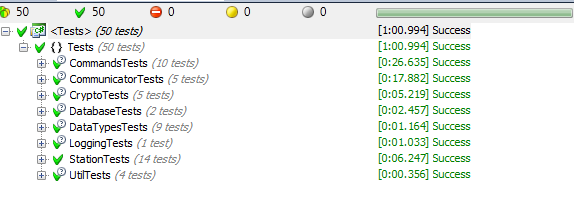
\includegraphics{TestRun.png}
\end{center}

The coverage results exclude parts of the system. It excludes some of the generated Entity Framework code, as we have not written it nor used it beyond what was covered.
We've also excluded some Finalize methods that were not being run due to IDisposable being implemented. The Finalize methods were not written by us, either. Some of the code was wrongfully marked as not being covered due to reasons unknown. This mostly covered lambda expressions in code contracts. \\

\textbf{Coverage results}
\begin{center}
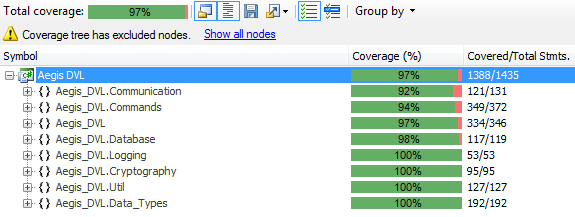
\includegraphics{CoverageWithoutFinalize.png}
\end{center}

\noindent 59/72 of the user interface blackbox tests passed. To view the tests in detail, see appendix \ref{sec:uitests} User interface tests. Most of these bugs are insignificant and can be easily repaired. They do not interrupt the normal workflow but are more of an inconvenience to the users. However, they should still be fixed before making the application publicly available since some of the bugs will crash the program completely.

\subsection{Known bugs}

Our testing revealed some bugs listed here: \\ \\

\noindent \begin{longtable}{|p{\textwidth-20mm}|p{15mm}|}
\multicolumn{2}{c}{Known bugs}

\\\hline
\bf Bug & \bf Severity

\\\hline
A station will never know it has been removed from the group, only the manager and all other stations will. & Major

\\\hline
When you add a station in the ManagerOverviewPage, it gets connected, but the election never starts as it is busy receiving the SyncCommand. & Major

\\\hline
"Random" IOExceptions : Unable to read data from the transport connection: An existing connection was forcibly closed by the remote host. & Major

\\\hline
You can promote a machine you are not connected to in the ManagerOverviewPage which results in the manager being lost. & Major

\\\hline
"Start valg" works, but the listener on the stations should not be busy executing other commands (like the SyncCommand after a public key-exchange), as it will not receive other commands during execution. & Major

\\\hline
If a station types in the proper password during a public key-exchange, but the manager cancels, then the station will have the manager's address and public key, but not the other way around. This will make following public key-exchange requests fail unless you re-create the station. & Minor

\\\hline
ElectNewManagerCommand should never be send to the manager. & Minor

\\\hline
You can only paste in 9 chars, and not the 10 of a CPR number in the UI. & Minor

\\\hline
We have on rare occasions experienced this exception on the manager machine: \emph{The CLR has been unable to transition from COM context 0x1b7ae0f0 to COM context 0x1b7ae340 for 60 seconds. The thread that owns the destination context/apartment is most likely either doing a non pumping wait or processing a very long running operation without pumping Windows messages. This situation generally has a negative performance impact and may even lead to the application becoming non responsive or memory usage accumulating continually over time. To avoid this problem, all single threaded apartment (STA) threads should use pumping wait primitives (such as CoWaitForMultipleHandles) and routinely pump messages during long running operations.}. 
It seems to mainly have been thread-deadlocking that has caused it, and we have not been able to consistently recreate it.
& Minor

\\\hline
If you click "Opdater" in the user interface while it is already updating, you will get an ObjectDisposedException. This is because the DiscoverNetworkMachines method uses the threadpool. & Minor

\\\hline
CPR numbers written in the user interface should be within the uint32 limits. Ideally, we should add more checks to the user interface, like making sure that the first two digits do not exceed 31, the next two digits do not exceed 12 and so on. & Minor

\\\hline
If multiple machines try to request the same ballot at the same time, only one is handed out, but no error message is shown on the other machines. & Minor

\\\hline
If you click "Marker v\ae lger" or "Afslut", any entered master password is considered wrong if you are in a window before the BallotRequestPage on a station or before the OverviewPage on the manager. & Minor

\\\hline
If you select an invalid key during load, an exception is thrown in the DataLoadPage. & Minor

\\\hline
If you try to add a station you are already connected to, an exception is thrown in the OverviewPage and ManagerOverviewPage. & Minor

\\\hline
When you have removed a station, the user interface list is not updated before you click "Opdater". & Minor

\\\hline
\end{longtable}

While most of the known bugs are minor and easily repairable we identified five major bugs. These bugs interrupts the normal workflow when using the application and must be fixed before using the application in a real world environment 

\chapter{Future Development}
When we started this project we were aware that gaining access to the government databases in Denmark was something that we did not want to pursue. We aimed to develop a system where another developer could easily adapt it to fit new database structures and communication method. To promote modularity and make it easy to exchange one part of the system without affecting other parts we made the following interfaces:
\begin{itemize}
\item ICommunicator
\item ICommand
\item ICrypto
\item IDatabase
\item IScanner
\item IDvlUi
\item ILogger
\end{itemize}
We also wanted to make a logging system where we logged as much information as possible. It could seem to be hard to find the information you are searching for, but with modern log analysis tools this can be achieved without too much of a hassle. We would rather log too much information and have future developers filter it, than log too little and force them to insert their own log statements all over the code.

\section{Improvements}
As a starting point for future development we have made a list of improvements would like to have done ourselves were we given more time:

\begin{itemize}
\item System
\begin{itemize}
\item For the system to be able to support letter votes prior to the election. This might benefit from having its own project and application but many of the principles discussed in this paper could be relevant.
\item Construct an easy way for users to access the log and filter it.
\item Be able to adjust the IP range and timeout for the DiscoverNetworkMachines method in Station from the user interface.
\item Make an installer that installs SQLite and a PDF reader, such as Adobe acrobat reader, along with the application. 
\item Modify the logging system to implement distributed logs instead of locally stored logs.
\item Modify the application in such a way that it would run as a service and require administrator rights to close.
\item Create a possibility to test the system before the election starts. Potentially done via a test voter.
\item Implement a message queue system in the manager communication layer.
\end{itemize}

\item User Interface
\begin{itemize}
\item Make sure that scanned voter number will be entered in the right text box regardless of focus.
\item For the user interface to be able to populate the lists of station in the OverviewPage and ManagerOverviewPage automatically and update it every ten seconds.
\item Remove the "Opdater" buttons on the OverviewPage and ManagerOverviewPage.
\item Make the "Tilf\o j", "Fjern" and "G\o r til Manager" buttons in the OverviewPage and ManagerOverviewPage inactive when nothing is selected, instead of the current solution when nothing happens when they are pressed.   
\item Bind the ''Enter'' key to the correct button in the ManagerOverviewPage dependant on which text boxes were filled.
\item For the user interface to be able to mark the correct station as not connected when the "Fjern" button is pressed in the OverviewPage and ManagerOverviewPage instead of populating the entire list again.
\item Construct a user interface for generating voter cards.
\item Make the AcceptManagerDialog, AcceptStationDialog and CheckMasterPasswordDialog focus the text box.
\end{itemize}
\end{itemize}

\chapter{Glossary}
\begin{description}

\item[Election venue] One of the venues where the election is held. Each venue has it own set of machines and election personnel.

\item[Station] A machine where voters can scan or type in their voter numbers and CPR numbers and are handed a ballot if they are eligible. 

\item[Manager] A machine that manages the stations in the network. The manager machine can add or remove stations from the network during the election. The election data is imported and exported from the manager machine. The manager machine is also responsible for starting and ending the election at the appropriate times.

\item[Voter] A person eligible for voting.

\item[Voter card] Each voter receives a voter card prior to the election. The voter card contain the voter number, name and election venue of the voter and is used to verify whether the voter is eligible to vote at a specific venue. When the voter wants to vote he has to present the voter card to receive a ballot.

\item[Voter number] A unique number identifying a specific voter during an election.

\item[Ballot] When a voter has been verified as eligible to vote he receives a ballot used to cast a vote.

\item[Election official] A normal poll worker that does not know the master password. The job of the election official is to hand out ballots to the eligible voters when the system has confirmed that it is OK. 

\item[Election secretary] The person responsible for a single election venue. Each election venue has one election secretary that holds the master password for that venue.

\item[Master password] A password generated before the election starts and held by the election secretary. It is used to start an election, end an election, register a voter only with his CPR number and access the log database.

\end{description}

\chapter{Reflection}
When designing a software solution that focuses on security one must be aware that no system is 100\% secure. Every time a new layer of security is added the responsibility is moved from one entity to another, whether this is a part of the system or an actual person (or multiple persons). It all comes down to which entities you trust. In this system we assume that the election secretary and the entity responsible for partitioning and collecting the data are both trustworthy sources. If any of these were to have malicious intent, they could easily jeopardize the election. This could be solved by adding a new layer of security and having a new entity control the privileges of the election secretary and the partitioning and gathering entity. This poses the problem of whether we trust the new controlling entity, and illustrates that adding additional layers of security is not always beneficial. \\

A desirable way to deal with this is distributed security. If several entities with different stakes control the security together it becomes more robust. As an example, a married couple might share a bank account. The husband does not trust the wife not to spend all the money on shoes, and the wife does not trust the husband not to spend it all on wine, but they need to be able to extract money from the bank account for shared needs. If they both have a part of the account password, they can only extract money from the account when both of them are present. This prevents each of them from emptying the bank account on their own. The same principle could be applied to the election venue, with members from opposing political parties, both not wanting the other to inappropriately manipulate the election.\\

When implementing the security in our system, we realized just how hard it actually is to implement, and how easy it is to implement it wrong. We initially considered using SSL and PGP/GPG with OpenSSL \cite{openssl} as using verified security approaches gives a greater sense of trust, but the documentation for OpenSSL.NET \cite{sslnet} was severely lacking. We eventually switched to using Bouncy Castle, where the documentation was better, but not great. Its greatest strength was probably the fact that it was a .NET implementation, and not merely a C wrapper, like OpenSSL.NET. In the end, we decided to implement our own secure communication. This was partially done due to not requiring all of the functionality of SSL or PGP/GPG, but also because of Bouncy Castle lacking some functionality, such as a SSL server, and the fact that the PGP/GPG implementation was clunky. Using a lot of the concepts of PGP/GPG, we do believe our secure communication is actually secure.

\chapter{Conclusion}
We believe the project has been a success. We successfully built a distributed digital voter list system with no single point of failure, that uses secure network communication and make use of encryption to secure personal sensitive data. The system was fully documented using the BON specification language, and was created using design by contract. A part of the system was also verified using the model checker UPPAAL. The system was also tested thoroughly, with a total of 97\% code coverage.
Though there are problems with the system that need to be fixed if it were to be used in a real election, the theory and design decisions are sensible and there is a solid foundation that can be developed from. With further development, we definitely believe the system could replace the system made by KMD. The primary requirements were fulfilled, and some of the secondary as well.\\

\bf Primary requirements: \rm
\begin{description}[style=nextline]

\item[Features] All of the requirements in this category were met. We have constructed a system with a graphical user interface where at least one manager machine and three station machines must be present.

\item[Code requirements] All of the testing and code requirements were met. The system is documented and tested using unit tests, black box tests and code contracts. 

\item[The system] All of the system requirements were met. The system is able to scan and print voter cards, it allows the extraction of the full data set at any given time during the execution of the application, and it allows voters to use any of the machines in the election venue.

\end{description}

\bf Secondary goals (optional): \rm
\begin{description}[style=nextline]

\item [It should be faster to use the system that using the current paper-based model.] We did not test the speed of our system compared to the current paper based system, but this could be an important metric when an optimal user interface is constructed. We advise that speed should be a part of the user test conducted when testing a new user interface.

\item [The system should be able to generate a list of all the voters of the election place and whether they have voted or not and print it.] This requirement was not met, and in retrospect it should not have been a goal. Our system has had a strong focus on security, and all the voter data is encrypted. Being able to print all the voter data could be considered a security flaw, and private sensitive data such as CPR numbers could needlessly be exposed. Nevertheless, the PDF generator code is able to generate a list of voter names and voter numbers, but this feature is never used.

\item [The graphical user interface should be easy to learn and use.] We did not test the usability of the user interface since it is only meant for demonstration purposes. If a new user interface is created, there should be a focus on the ease of learning and ease of use. 

\item [The system should support letter votes.] This requirement was not met, but the possibility for gathering the letter votes beforehand and passing the voter data to our system is present, thereby eliminating the need to merge the data later on. However, this would require that the letter votes were partitioned in the same way as the voter data for each election venue.

\item [Use a data flow analysis tool to reason about correctness of the data flow in the system.] We used the model checking tool UPPAAL \cite{uppaal} to reason about the synchronization algorithm in the system. UPPAAL could also be used to reason about additional parts of the system to ensure its correctness.

\item [Use an analysis tool to reason about the cryptographic protocol used.] This requirement was not met, but would be a great addition to the security guarantee the system provides.

\end{description}


\begin{thebibliography}{9}
\bibitem{basin} Applied information security: A hands-on approach - David Basin, Patrick Schaller, Michael Schl{\"a}pfer - Springer-Verlag Berlin Heidelberg 2001

\bibitem{lynch} Distributed Algorithms - Nancy A. Lynch - Morgan Kaufmann Publishers Inc. 1996

\bibitem{bakshi} Leader Election Algorithm in Anonymous Rings: Franklin Goes Probabilistic - Rena Bakhshi - Milan, September 9, 2008 - retrieved from \url{http://www.few.vu.nl/~rbakhshi/papers/TCS08talk.pdf} on 12th March 2012

\bibitem{aiello} Leader Election in rings - Marco Aiello, Eirini Kaldeli - University of Groningen 2009 - retrieved from \url{http://www.cs.rug.nl/~eirini/DS_slides/leader_election.pdf} on 12th March 2012

\bibitem{moore} Attack Modeling for Information Security and Survivability - Andrew P. Moore,
Robert J. Ellison, Richard C. Linger - March 2001 - retrieved from 
\url{http://www.cert.org/archive/pdf/01tn001.pdf} on 12th March 2012

\bibitem{schneier} Attack Trees: Modeling security threats - Bruce Schneier - Dr. Dobb's Journal December 1999 - retrieved from \url{http://www.schneier.com/paper-attacktrees-ddj-ft.html} on 12th March 2012

\bibitem{tree} Creating Secure Systems through  Attack Tree Modeling – 10 June 2003 - retrieved from \url{http://www.amenaza.com/downloads/docs/5StepAttackTree_WP.pdf} on 12th March 2012

\bibitem{meier} Improving Web Application Security: Threats and Countermeasures - J.D. Meier, Alex Mackman, Michael Dunner, Srinath Vasireddy, Ray Escamilla and Anandha Murukan - Microsoft Corporation June 2003 - retrieved from \url{http://msdn.microsoft.com/en-us/library/ff648644.aspx} on 12th March 2012

\bibitem{shmueli} Database Encryption: An Overview of Contemporary Challenges and Design Considerations - Erez Shmueli, Ronen Vaisenberg, Yuval Elovici, Chanan Glezer - SIGMOD Record, September 2009 - retrieved from \url{http://www.ics.uci.edu/~ronen/Site/Research_files/p29.surveys.shmueli.pdf} on 12th March 2012

\bibitem{dbmscrypto} 24 DBMS\_CRYPTO - Oracle® Database PL/SQL Packages and Types Reference 10g Release 2 (10.2) Part Number B14258-02 - retrieved from \url{http://docs.oracle.com/cd/B19306_01/appdev.102/b14258/d_crypto.htm} on 12th March 2012

\bibitem{hsueh} Database Encryption in SQL Server 2008 Enterprise Edition
- Sung Hsueh - Microsoft, February 2008 - retrieved from \url{http://msdn.microsoft.com/en-us/library/cc278098(v=sql.100).aspx} on 12th March 2012

\bibitem{kiely} Protect Sensitive Data Using Encryption in SQL Server 2005 - Don Kiely - Microsoft, December 2006 - retrieved from \url{download.microsoft.com/download/4/7/a/47a548b9-249e-484c-abd7-29f31282b04d/SQLEncryption.doc} on 12th March 2012

\bibitem{mysqlcrypt} 11.13. Encryption and Compression Functions - retrieved from \url{http://dev.mysql.com/doc/refman/5.5/en/encryption-functions.html} on 12th March 2012

\bibitem{access} Encrypting an Access Database - Mike Chapple - retrieved from \url{http://databases.about.com/od/productinfo/a/encryption.htm} on 12th March 2012

\bibitem{postgre} PostgreSQL 8.1.23 Documentation : 16.6. Encryption Options - retrieved from \url{http://www.postgresql.org/docs/8.1/static/encryption-options.html} on 12th March 2012

\bibitem{sqliteee} The SQLite Encryption Extension (SEE) - retrieved from \url{http://www.hwaci.com/sw/sqlite/see.html} on 12th March 2012

\bibitem{sqlite} SQLite Home Page - retrieved from \url{http://www.sqlite.org} on 18th March 2012

\bibitem{firebird} How to protect data in Firebird database? - retrieved from \url{http://www.firebirdfaq.org/faq160/} on 12th March 2012

\bibitem{sybase} Adaptive Server Enterprise 15.0 > ASE 15.0 with Encrypted Columns - retrieved from \url{http://infocenter.sybase.com/help/index.jsp?topic=/com.sybase.dc00412_1500/html/Encrypt_Guide/BAJCAIHA.htm} on 12th March 2012

\bibitem{db2} Encrypting Data Values in DB2 Universal Database - Bruce Benfield, Richard Swagerman - International Business Machines Corporation, 2001 - retrieved from \url{http://www.ibm.com/developerworks/data/library/techarticle/benfield/0108benfield.html} on 12th March 2012

\bibitem{mongo} MongoDB - retrieved from \url{http://www.mongoDB.org} on 19th March 2012

\bibitem{couch} The Apache CouchDB Project - retrieved from \url{http://couchdb.apache.org/} on 19th March 2012

\bibitem{redis} Redis - retrieved from \url{http://redis.io} on 19th March 2012

\bibitem{chandy} Distributed snapshots: determining global states of distributed systems - K. Mani Chandy \& Leslie Lamport - ACM Transactions on Computer Systems, Vol. 3, No. 1, February 1965. - retrieved from \url{http://research.microsoft.com/en-us/um/people/lamport/pubs/chandy.pdf} on 10th April 2012

\bibitem{schooler} Why Multicast Protocols (Don't) Scale : An Analysis of Multipoint Algorithms for Scalable Group Communication - Eve M. Schooler - California Institute of Technology, 2001 - retrieved from \url{http://thesis.library.caltech.edu/3236/11/thesis.pdf} on 10th April 2012

\bibitem{nsync} SyncAlgorithm - retrieved from \url{http://code.google.com/p/nsync/wiki/SyncAlgorithm} on 10th April 2012

\bibitem{logcomp} Comparison of .NET Logging Frameworks and Libraries - retrieved from \url{http://www.dotnetlogging.com/comparison/} on 16th April 2012

\bibitem{uppaal} UPPAAL home - retrieved from \url{http://www.uppaal.org/} on 7th May 2012

\bibitem{dvrs} Digital Voter Registration System - Christian Olsson, K\aa re Sylow Pedersen and Henrik Haugb\o lle - IT University of Copenhagen, 14th December 2011 

\bibitem{nunit} NUnit Home - retrieved from \url{http://www.nunit.org/} on 8th May 2012

\bibitem{dotcover} Code coverage tool for .NET :: dotCover \url{http://www.jetbrains.com/dotcover/} on 11th May 2012

\bibitem{pex} Pex, Automated White box Testing for .NET - retrieved from \url{http://research.microsoft.com/en-us/projects/pex/default.aspx} on 18th May 2012

\bibitem{bon} Business Object Notation (BON) - Kim Waldén, Enea Data - Chapter 10 in ''Handbook of Object Technology'', CRC Press 1998 - retrieved from \url{http://www.bon-method.com/handbook_bon.pdf} on 10th May 2012

\bibitem{codec} Code Contracts - retrieved from \url{http://msdn.microsoft.com/en-us/library/dd264808.aspx} on 10th May 2012

\bibitem{dbc} Applying ''Design By Contract'' - Bertrand Meyer - October 1992 - retrieved from \url{http://se.ethz.ch/~meyer/publications/computer/contract.pdf} on 10th May 2012

\bibitem{kmd1}Systembeskrivelse KMD Digital Valgliste Version 2.1.0 - KMD A/S 05-09-2011 - retrieved from \url{http://nykundenet.kmd.dk/systembrugere/valg/Valgudskrivning/Vejledninger/Digital%20Valgliste.%20Systembeskrivelse.%20Version%202.1.0.pdf} on 10th May 2012

\bibitem{kmd2} Kom godt i gang KMD Digital Valgliste. Tekniker Version 2.1.0 - KMD A/S 05-09-2011 - retrieved from \url{http://nykundenet.kmd.dk/systembrugere/valg/Valgudskrivning/Vejledninger/Kom%20godt%20i%20gang.%20Digital%20Valgliste.%20Tekniker.%20Version%202.1.0.pdf} on 10th May 2012

\bibitem{kmd3} Installationsvejledning til KMD Digital Valgliste Konfiguration Version 2.2 - KMD A/S - retrieved from \url{http://nykundenet.kmd.dk/systembrugere/valg/Valgudskrivning/Vejledninger/Installationsvejledning%20til%20KMD%20Digital%20Valgliste%20Konfiguration%20Version%202.2.pdf} on 10th May 2012

\bibitem{gloss} E-Voting Technology Glossary - retrieved from \url{http://whatis.techtarget.com/glossary/e-voting-glossary.html} on 11th May 2012

\bibitem{punch} Punchscan see your vote count - retrieved from \url{http://www.punchscan.org/} on 11th May 2012

\bibitem{scant} Scantegrity - retrieved from \url{http://www.scantegrity.org/} on 11th May 2012

\bibitem{domi} Dominion Voting is a different kind of election partner - retrieved from \url{http://www.dominionvoting.com/} on 11th May 2012

\bibitem{medi} Mediator Design Pattern in C\# and VB.NET - retrieved from \url{http://www.dofactory.com/Patterns/PatternMediator.aspx} on 15th May 2012

\bibitem{pgp} The International PGP Home Page - retrieved from \url{http://www.pgpi.org/} on 15th May 2012

\bibitem{cmdp} Command Design Pattern in C\# and VB.NET - retrieved from \url{http://www.dofactory.com/Patterns/PatternCommand.aspx} on 15th May 2012

\bibitem{four} Four-eye principle / Planning and organization - retrieved from \url{http://www.economypoint.org/f/four-eye-principle.html} on 15th May 2012

\bibitem{adonet} ADO.NET 2.0 Provider for SQLite - retrieved from \url{http://sourceforge.net/projects/sqlite-dotnet2/} on 18th May 2012

\bibitem{orm} What is object-relational mapping (ORM)? -  retrieved from \url{http://searchwindevelopment.techtarget.com/definition/object-relational-mapping} on 18th May 2012

\bibitem{gpg} The GNU Privacy Guard - retrieved from \url{http://www.gnupg.org/} on 18th May 2012

\bibitem{ssl} What is SSL? SSL Certificate Basics - retrieved from \url{http://www.sslshopper.com/what-is-ssl.html} on 18th May 2012

\bibitem{bouncy} The Legion of the Bouncy Castle C\# Cryptography APIs - retrieved from \url{http://www.bouncycastle.org/csharp/} on 18th May 2012

\bibitem{rsa} RSA Algorithm - retrieved from \url{http://www.di-mgt.com.au/rsa_alg.html} on 18th May 2012

\bibitem{oaep} Optimal Asymmetric Encryption: How to Encrypt with RSA - Mihir Bellare, Phillip Rogaway - Springer-Verlag, 19. nov 1995 - retrieved from \url{http://cseweb.ucsd.edu/users/mihir/papers/oae.pdf} on 18th May 2012

\bibitem{aes} AES Explained - retrieved from \url{http://x-n2o.com/aes-explained} on 18th May 2012

\bibitem{cbc} Secure Programming Cookbook for C and C++, section 5.4.3.2 - Matt Messier, John Viega - O'Reilly - July 2003

\bibitem{pkcs7} PKCS \#7: Cryptographic Message Syntax - retrieved from \url{http://tools.ietf.org/html/rfc2315} on 18th May 2012

\bibitem{ccm} Secure Programming Cookbook for C and C++, section 5.4 - Matt Messier, John Viega - O'Reilly - July 2003

\bibitem{rsastr} Recommendation for Key Management Part 1: General (Revised) - Elaine Barker, William Barker, William Burr, William Polk, Miles Smid - NIST Special Publication March 2007 - retrieved from \url{http://csrc.nist.gov/publications/nistpubs/800-57/sp800-57-Part1-revised2_Mar08-2007.pdf} on 21th May 2012

\bibitem{aesstr} How secure is AES against brute force attacks? - Mohit Arora - retrieved from \url{http://www.eetimes.com/design/embedded-internet-design/4372428/How-secure-is-AES-against-brute-force-attacks-} on 21th May 2012

\bibitem{openssl} OpenSSL: The Open Source toolkit for SSL/TLS - retrieved from \url{http://www.openssl.org/} on 22th May 2012


\bibitem{sslnet} OpenSSL.NET - retrieved from \url{http://openssl-net.sourceforge.net/} on 22th May 2012

\end{thebibliography}

\chapter{Appendix}

\section{User interface tests}
\label{sec:uitests}
\noindent \begin{longtable}{|p{5mm}|p{\textwidth / 4}|p{\textwidth / 4}|p{\textwidth / 4}|p{\textwidth / 4}|}
\multicolumn{4}{c}{UI Tests}
\\\hline
\bf No & \bf Task & \bf Expected Behavior & \bf Did it behave as expected & \bf Errors

\\\hline
- & TypeChoicePage & - & - & - 

\\\hline
1 & Push the Station button on the TypeChoicePage & Redirection to the WaitingForManagerPage & Yes & None 

\\\hline
2 & Push the Manager button on the TypeChoicePage & Redirection to the MasterPasswordPage & Yes & None 

\\\hline
3 & Push the Afslut button on the TypeChoicePage & The application closes & Yes & None 

\\\hline
- & Menus & - & - & - 

\\\hline
4 &Choose User manual under the Help menu & the user manual opens as a .pdf file & Yes & None 

\\\hline
5 & Choose Exit under the File menu & A prompt asks for the master password and the application closes if it correct & No & The master password is always be false if you are in TypeChoicePage, WaitingForManagerPage, MasterPasswordPage and DataLoadPage. This is becsuse the station object have not been initialized.

 \\\hline
6 & Choose Export Data under the File Menu & two prompt appears, one asking for the master password and one asking for the destination of the data. If both are valid the data is exported to the location. & Yes & None 

 \\\hline
7 & Choose Mark Voter under the File Menu & two prompts appears one allowing you to type the CPR number of a voter and one asking you for the master password. If the master password is correct a prompt shows whether or not the voter is eligible for a ballot & Yes & None 

\\\hline
- & DataLoadPage & - & - & -

\\\hline
8 & Press N\ae ste on the DataLoadPage with data and key selected in the right format & redirection to the OverviewPage & Yes & None 

\\\hline
9 & Press N\ae ste on the DataLoadPage with data selected in the right format but the key in the wrong format & A prompt telling you the import was not successful & No & An Exception is thrown

\\\hline
10 & Press N\ae ste on the DataLoadPage with both data  and key selected in the wrong format & A prompt telling you the import was not successful & No & An Exception is thrown

\\\hline
11 & Press N\ae ste on the DataLoadPage with key selected in the right format but the data in the wrong format & A prompt telling you the import was not successful & Yes & None

\\\hline
12 & Press N\ae ste on the DataLoadPage with no key and no data selected & A prompt telling you the import was not successful & Yes & None

\\\hline
13 & Pressing the Tilbage button on the DataLoadPage & redirection to the TypeChoicePage & Yes & None

 \\\hline
- & MasterPasswordPage & - & - & - 

\\\hline
14 & Entering the MasterPasswordPage & a random generated password is shown & Yes & None

\\\hline
15 & Pressing Tilbage on the MasterPasswordPage & redirection to the TypeChoicePage & Yes & None 

\\\hline
16 & Pressing N\ae ste on the MasterPasswordPage  & redirection to the DataLoadPage & Yes & None 

\\\hline
- & WaitingForManagerPage & - & - & - 

 \\\hline
17 & While on the WaitingForManagerPage a manager tries to connect & A prompt asking for a password to be typed appears. If this is correct a similar prompt appears on the manager and the password is shown on the station & Yes & None 

 \\\hline
18 & While on the WaitingForManagerPage a manager is connected & The Page displays the text Venter p\aa  at valget starter & Yes & None 

 \\\hline
19 & While on the WaitingForManagerPage the election is started & redirection to BallotRequestPage & Yes & None 

 \\\hline
20 & Press Tilbage while on WaitingForManagerPage & redirection to TypeChoicePage & Yes & None 

\\\hline
- & BallotRequestPage & - & - & -

 \\\hline
21 & Press F\ae rdig with a valid voter number and CPR number in the appropriate text boxes & A prompt saying that the voter can be handed a ballot appears & Yes & None 

 \\\hline
22 & Press F\ae rdig with an invalid voter number and CPR number in the appropriate text boxes & A prompt saying that the voter can not be handed a ballot appears & Yes & None 

 \\\hline
23 & Press F\ae rdig with a valid voter number and but an invalid CPR number in the appropriate text boxes & A prompt saying that the voter can not be handed a ballot appears & Yes & None 

 \\\hline
24 & Press F\ae rdig with an invalid voter number and a valid CPR number in the appropriate text boxes & A prompt saying that the voter can not be handed a ballot appears & Yes & None 

\\\hline
25 & Press F\ae rdig with no voter number and a valid CPR number in the appropriate text boxes & You can not press the F\ae rdig button & Yes & None 

\\\hline
26 & Press F\ae rdig with a valid voter number and no CPR number in the appropriate text boxes & You can not press the F\ae rdig button & Yes & None 

\\\hline
27 & Press F\ae rdig with no voter number and no CPR number in the appropriate text boxes & You can not press the F\ae rdig button & Yes & None 

\\\hline
28 & Press F\ae rdig with a valid voter number and a valid CPR number in the appropriate text boxes, that has already voted & A prompt saying that the voter can not be handed a ballot appears & Yes & None 

\\\hline
29 & Press F\ae rdig with a valid voter number and a valid CPR number in the appropriate text boxes but not enough stations are connected & You can not press the F\ae rdig button and a label showing that not enough stations are connected appears & Yes & None 

\\\hline
- & EndedElectionPage & - & - & -    

 \\\hline
30 & Press the Gennemse button in the EndedElectionPage & a file browser appears and lets you choose a destination, if you do notchoose one nothing appears in the text box & Yes & None 

 \\\hline
31 & Press the Eksporter button with no destination selected in the EndedElectionPage & you can not press the Eksporter button & Yes & None 

 \\\hline
32 & Press the Eksporter button with a destination selected in the EndedElectionPage & The data is exported to the selected destination & Yes & None 

\\\hline
- & OverviewPage & - & - & -

 \\\hline
33 & Press the Opdater button in the OverviewPage & A progress bar appears indicating that the list is updating. When it is done the list is updated  & Yes & None 

 \\\hline
34 & Press the Opdater Button in the OverviewPage while it is updating & the old update is canceled and a new update of the list starts & No & a ObjectDisposedException is thrown

 \\\hline
35 & Press the Tilbage button in the OverviewPage & redirection to the DataLoadPage & Yes & None

 \\\hline
36 & Press the Tilf\o j button with nothing selected in the OverviewPage & Nothing happens & Yes & None

 \\\hline
37 & Press the Fjern button with nothing selected in the OverviewPage & Nothing happens & Yes & None

 \\\hline
38 & Press the Tilf\o j button with a station you are already connected to, selected in the OverviewPage & Nothing happens & No & an Exception is thrown

 \\\hline
39 & Press the Fjern button with a station you are not connected to, selected in the OverviewPage & Nothing happens & Yes & None

 \\\hline
40 & Press the Tilf\o j button with a station you are not connected to, selected in the OverviewPage & a password appears on the screen and a prompt to type in this password appears on the station & Yes & None 

 \\\hline
41 & A station replies to your request to add it in the OverviewPage & a prompt appears on your screen and if you type in the correct password the station appears as connected in the list & Yes & None 

\\\hline
42 & Press the Fjern button with a station you are connected to, selected in the OverviewPage & The station appears as not connected in the list & No & while it is removed, it appears in the list as not connected only after the list has been updated. 

\\\hline
43 & Press the Start Valg button in the OverviewPage while you are connected to an amount of stations less than the required amount & a box appears telling you that you can not start the election without connecting to more machines & Yes & None 

\\\hline
44 & Press the Start Valg button in the OverviewPage while you are connected to the required amount of stations or more & redirection to the ManagerOverviewPage. All the connected stations redirected to the BallotRequestPage & Yes & None 

\\\hline
- & ManagerOverviewPage & - & - & -

 \\\hline
45 & Press F\ae rdig with a valid voter number and CPR number in the appropriate text boxes & A prompt saying that the voter can be handed a ballot appears & Yes & None 

 \\\hline
46 & Press F\ae rdig with an invalid voter number and CPR number in the appropriate text boxes & A prompt saying that the voter can not be handed a ballot appears & Yes & None 

 \\\hline
47 & Press F\ae rdig with a valid voter number and but an invalid CPR number in the appropriate text boxes & A prompt saying that the voter can not be handed a ballot appears & Yes & None 

 \\\hline
48 & Press F\ae rdig with an invalid voter number and a valid CPR number in the appropriate text boxes & A prompt saying that the voter can not be handed a ballot appears & Yes & None 

\\\hline
49 & Press F\ae rdig with no voter number and a valid CPR number in the appropriate text boxes & You can not press the F\ae rdig button & No & A prompt appears saying that voter can not receive a ballot

\\\hline
50 & Press F\ae rdig with a valid voter number and no CPR number in the appropriate text boxes & You can not press the F\ae rdig button & Yes & None

\\\hline
51 & Press F\ae rdig with no voter number and no CPR number in the appropriate text boxes & You can not press the F\ae rdig button & Yes & None

\\\hline
52 & Press F\ae rdig with a valid voter number and a valid CPR number in the appropriate text boxes, that has already voted & A prompt saying that the voter can not be handed a ballot appears & Yes & None 

\\\hline
53 & Press F\ae rdig with a valid voter number and a valid CPR number in the appropriate text boxes but not enough stations are connected & You can not press the F\ae rdig button and a label showing that not enough stations are connected appears & Yes & None 

 \\\hline
54 & Press Kun CPR with a valid CPR number in the appropriate text box & A prompt saying that the voter can be handed a ballot appears after you have typed the master password & Yes & None 

 \\\hline
55 & Press Kun CPR with an invalid CPR number in the appropriate text box & A prompt saying that the voter can not be handed a ballot appears after you have typed the master password & Yes & None 

\\\hline
56 & Press F\ae rdig with no CPR number in the appropriate text box & You can not press the Kun CPR button & Yes & None

\\\hline
57 & Press Kun CPR with a valid CPR number in the appropriate text boxes but not enough stations are connected & You can not press the Kun CPR button and a label showing that not enough stations are connected appears & Yes & None 

 \\\hline
58 & Press the Opdater button in the ManagerOverviewPage & A progress bar appears indicating that the list is updating. When it is done the list is updated  & Yes & None 

 \\\hline
59 & Press the Opdater Button in the ManagerOverviewPage while it is updating & the old update is canceled and a new update of the list starts & No & a ObjectDisposedException is thrown

 \\\hline
60 & Press the Tilf\o j button with nothing selected in the ManagerOverviewPage & Nothing happens & Yes & None

 \\\hline
61 & Press the Fjern button with nothing selected in the ManagerOverviewPage & Nothing happens & Yes & None

 \\\hline
62 & Press the Tilf\o j button with a station you are already connected to, selected in the ManagerOverviewPage & Nothing happens & No & an Exception is thrown

 \\\hline
63 & Press the Fjern button with a station you are not connected to, selected in the ManagerOverviewPage & Nothing happens & Yes & None

 \\\hline
64 & Press the Tilf\o j button with a station you are not connected to, selected in the ManagerOverviewPage & a password appears on the screen and a prompt to type in this password appears on the station & Yes & None 

 \\\hline
65 & A station replies to your request to add it in the ManagerOverviewPage & a prompt appears on your screen and if you type in the correct password the station appears as connected in the list. The station is redirected to the BallotRequestPage & No & the station is never redirected to the BallotRequestPage 

\\\hline
66 & Press the Fjern button with a station you are connected to, selected in the ManagerOverviewPage & The station appears as not connected in the list & No & while it is removed, it appears in the list as not connected only after the list has been updated. 

\\\hline
67 & Press the G\o r til Manager button while nothing is selected in the ManagerOverviewPage & Nothing happens & Yes & None 

\\\hline
68 & Press the G\o r til Manager button while a station you are not connected to, is selected in the ManagerOverviewPage & Nothing happens & No & The station never gets promoted but the manager gets demoted to a station 

\\\hline
69 & Press the G\o r til Manager button while a station you are connected to, is selected in the ManagerOverviewPage & the manager gets demoted to at station and the station becomed the new manager. Redirect to BallotRequestPage for manager and redirect to ManagerOverviewPage for station & Yes & None

\\\hline
70 & Press the Afslut Valg button int he ManagerOverviewPage & after having typed the correct master password, redirect to the EndedElectionPage. All stations close their applications & Yes & None 

\\\hline
- & Election and crashes & - & - & -

\\\hline
71 & During the election, sever the connection to the manager & a new manager is elected and promoted & No & a new manager is elected correctly but not at the time the severing occurs, but on the next action requiring network traffic taken by any station.

\\\hline
72 & During the election, sever the connection to a station & the station is removed from the managers list of peers & Yes & None

\\\hline
\end{longtable}

\section{Class diagrams}
\label{sec:classd}
\subsection*{ Aegis DVL - All}
\begin{center}
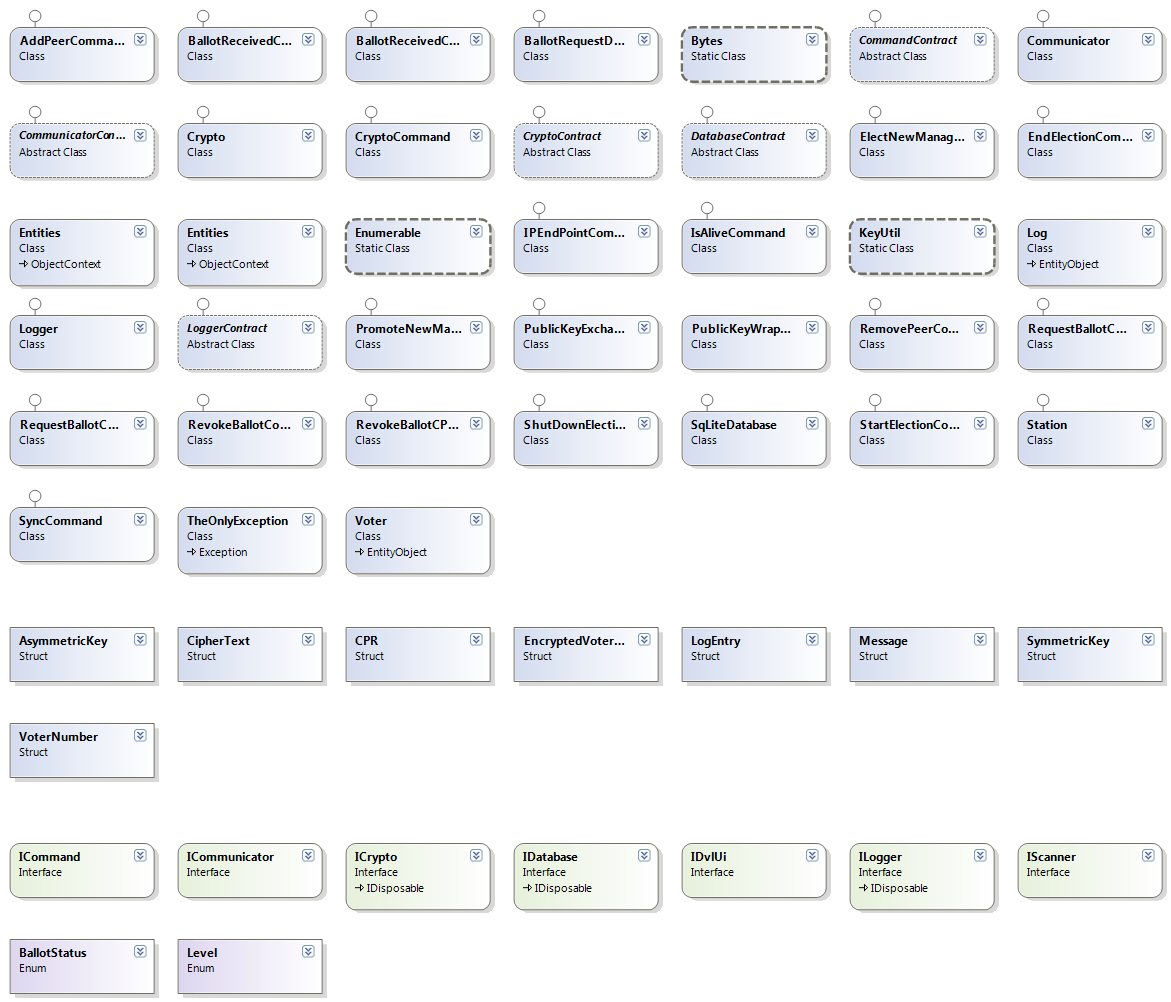
\includegraphics[width=\textwidth]{DVLClassdiagram_All.png}
\end{center}
\subsection*{ Aegis DVL - Commands and Communication}
\begin{center}
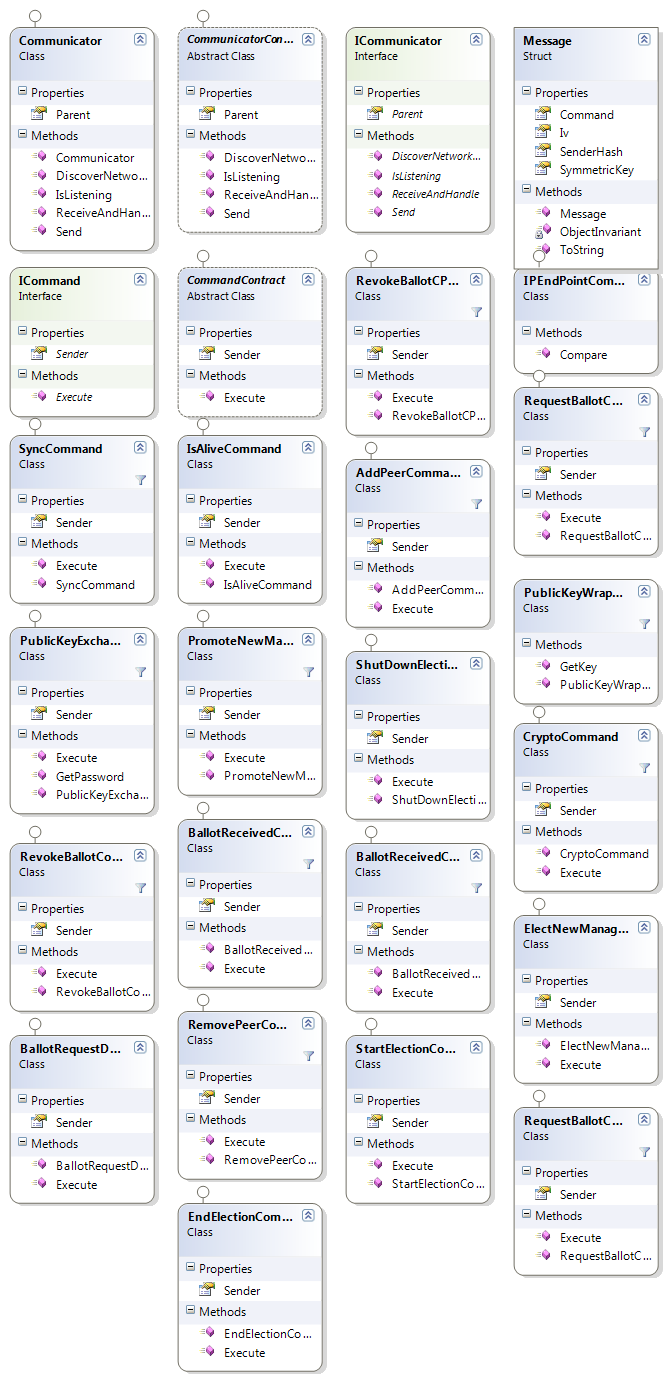
\includegraphics[width=\textwidth, height=\textheight - 10mm]{DVLClassdiagram_Commands.png}
\end{center}
\subsection*{ Aegis DVL - Database}
\begin{center}
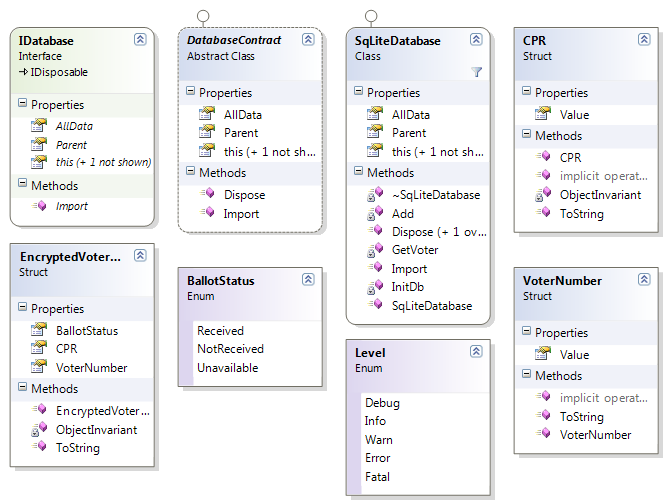
\includegraphics[width=\textwidth]{DVLClassdiagram_Database.png}
\end{center}
\subsection*{ Aegis DVL - Logging}
\begin{center}
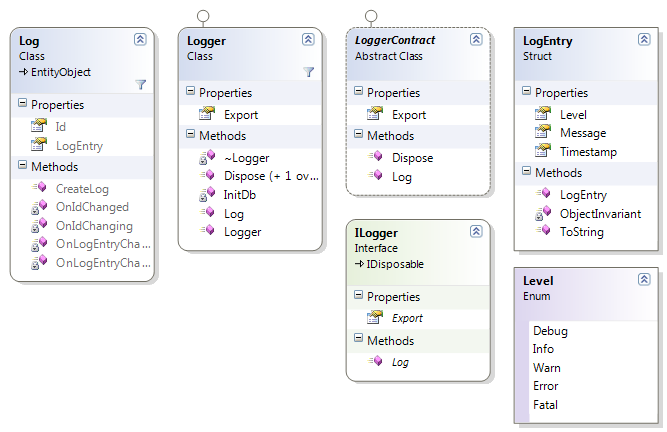
\includegraphics[width=\textwidth]{DVLClassdiagram_Logging.png}
\end{center}
\subsection*{ Aegis DVL - Crypto}
\begin{center}
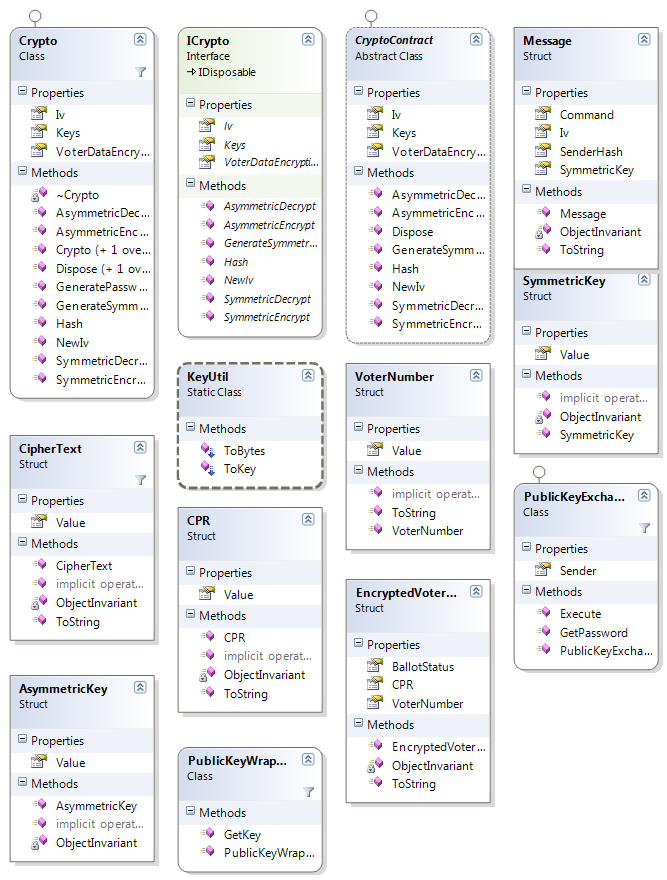
\includegraphics[width=\textwidth]{DVLClassdiagram_Crypto.png}
\end{center}
\subsection*{ Aegis DVL User interface - All}
\begin{center}
\includegraphics[width=\textwidth]{UIClassdiagram_All.png}
\end{center}
\subsection*{ Aegis DVL User interface - Station}
\begin{center}
\includegraphics[width=\textwidth]{UIClassdiagram_Station.png}
\end{center}
\subsection*{ Aegis DVL User interface - Manager}
\begin{center}
\includegraphics[width=\textwidth]{UIClassdiagram_Manager.png}
\end{center}
UI
Commands
Back end
Tests
\section{User manual}
\label{sec:uman}
\subsection*{Installation}
\begin{enumerate}
\item Before the election a manager machine should be placed away from the voters and all the station machines should be placed so that they are accessible to the voters.
\item Install the ADO.NET 2.0 Provider for SQLite, (link \url{http://sourceforge.net/projects/sqlite-dotnet2/}) on each machine. This is the database framework needed to run the program.
\item Install Adobe acrobat reader, (link \url{http://get.adobe.com/reader/}) or another PDF reader on each machine. The user manual in the program is a PDF file and Adobe acrobat reader is able to display it.
\item Make sure that each machine is in the 192.168.0.1 - 192.168.255.255 IP range.
\item When using this application for the first time Windows will ask you if you want to allow Aegis DVL to pass through your firewall. You need to allow this.
\item Start the Digital Voter List application on each of the machines.
\item You are now presented with this screen: \\
\begin{center}
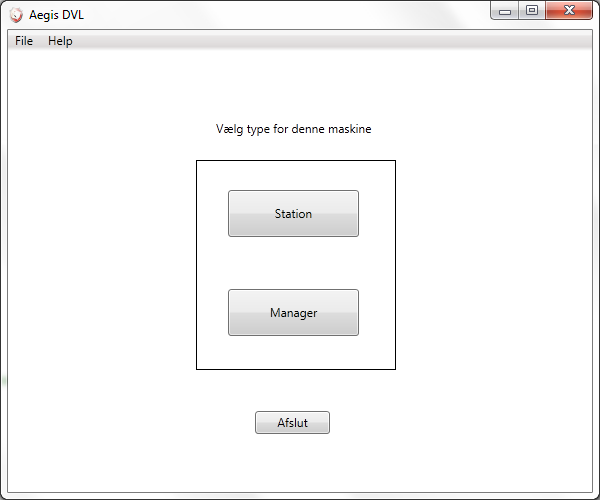
\includegraphics[width=100mm]{TypeChoice.png}
\end{center}
Choose Manager on the manager machine and Station on all the station machines.
\end{enumerate}

\subsection*{Station usage}
\begin{enumerate}
\item After you have selected Station you are presented with this page: \\
\begin{center}
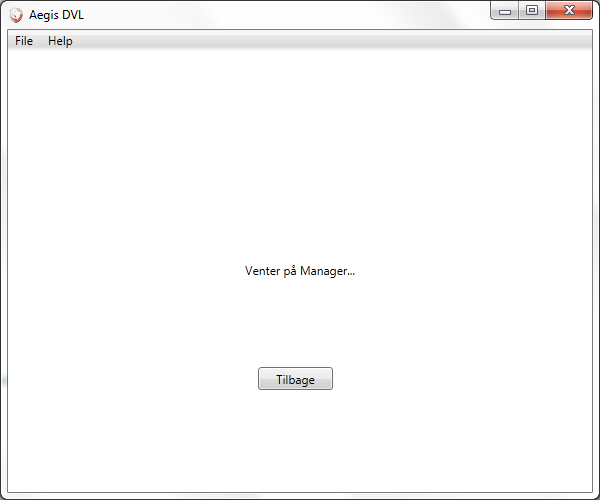
\includegraphics[width=100mm]{WaitingForManager.png}
\end{center}
This screen is displayed until a manager connects.
\item When a manager connects a password is shown on his screen and you are presented with this screen: \\
\begin{center}
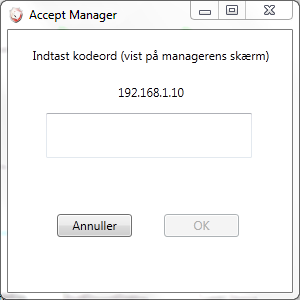
\includegraphics{AcceptManagerDialog.png}
\end{center}
Type the password displayed on the manager in this window and press OK.
\item When the password has been accepted, the reverse process begins. Now a password is displayed on your screen like this: \\
\begin{center}
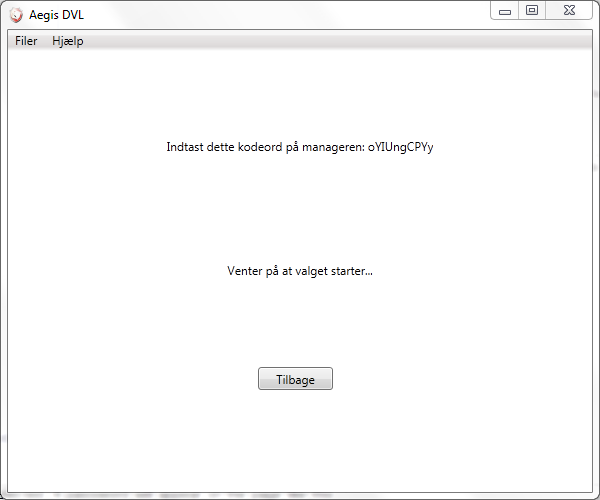
\includegraphics[width=100mm]{WaitingForManagerWithPassword.png}
\end{center}
Have the manager type this password in and the text on your screen switches to "Venter p\aa      \ at valget starter" which is displayed until the manager decides to start the election.
\item When the election starts you are presented with this screen: \\
\begin{center}
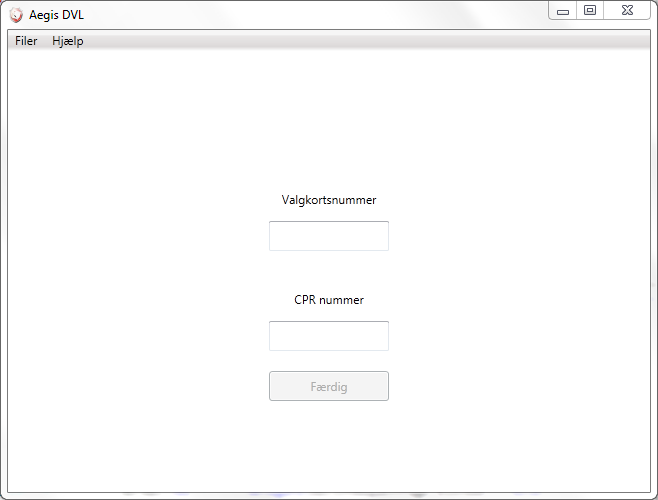
\includegraphics[width=100mm]{BallotRequest.png}
\end{center}
From this screen voters can scan/type their voter numbers and type in their CPR numbers. When this is done you can press "F\ae rdig" and one of the following dialogues is shown: \\
\begin{center}
 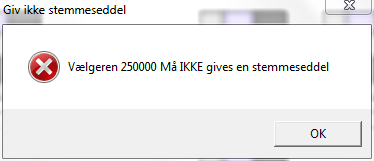
\includegraphics{BallotDenied.png}
\end{center}
This indicates that the voter is either not eligible to vote at this venue or that he has already been handed a ballot. \\
\begin{center}
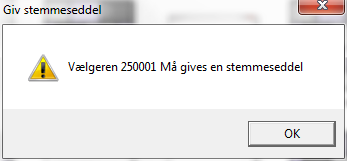
\includegraphics{BallotAccepted.png}
\end{center}
This indicates that the system has accepted the voter number and CPR number and that this voter can now be handed a ballot.
\item This process can be repeated until the manager decides that the election has ended.
\item When the election has ended the application automatically shuts down.
\item When the manager has exported the data and everyone is sure that the election has run as expected it is safe to delete the Voters.data file.
\end{enumerate}

\subsection*{Manager usage}
\begin{enumerate}
\item After you have selected Manager you are presented with this page: \\
\begin{center}
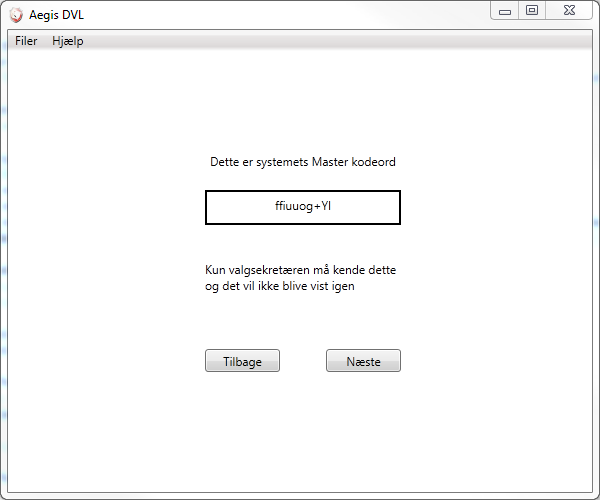
\includegraphics[width=100mm]{MasterPassword.png}
\end{center}
This window displays the master password. It should only be read by the election secretary and is never shown again! It is used to start an election, end an election, register a voter only with his CPR number and access the log database.
\item When you press "N\ae ste" you are presented with the Data Load Page: \\
\begin{center}
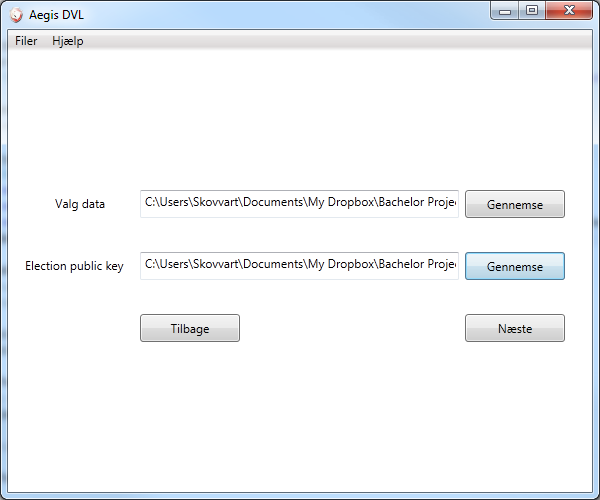
\includegraphics[width=100mm]{DataLoad.png}
\end{center}
From here you can choose the file location of the voter data the system needs to import and the encryption key for the voter data in question. When you have found these press "N\ae ste".
\item You are now presented with this page: \\
\begin{center}
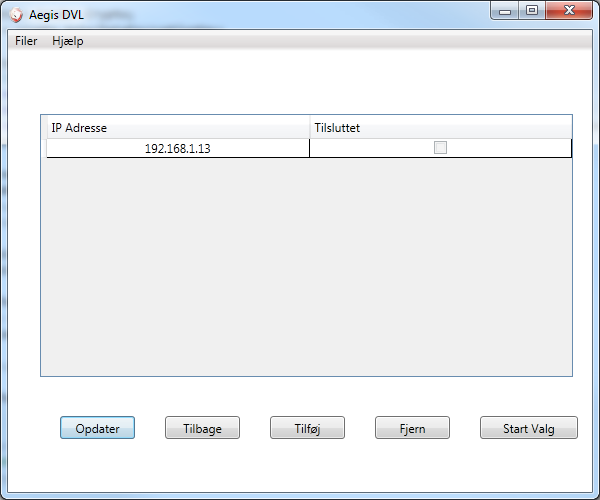
\includegraphics[width=100mm]{Overview.png}
\end{center}
From here you have several options. "Opdater" updates the list of stations you can connect to. "Tilbage" takes you back to the page showing the data loading. It generates a new master password which should be used henceforth. "Tilf\o j" attempts to connect to the station you have selected. A password appears on the page like this: \\
\begin{center}
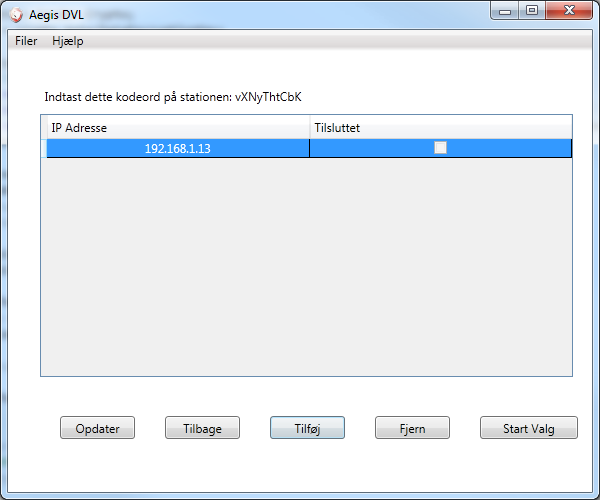
\includegraphics[width=100mm]{OverviewWithPassword.png}
\end{center}
and the station needs to input the password. After the station has entered the password and pressed "OK" you are asked for a password displayed on the station like this:
\begin{center}
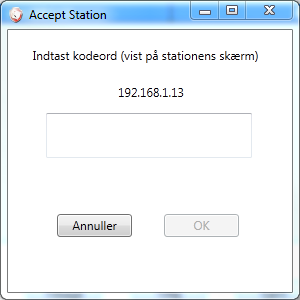
\includegraphics{AcceptStationDialog.png}
\end{center}
When you enter the right password the station appears as connected in the list. Pressing "Fjern" removes the stations as a peer, and announces to the remaining peers that they must do the same. A removed peer is ignored. "Start valg" asks you for the master password and start the election like so: \\
\begin{center}
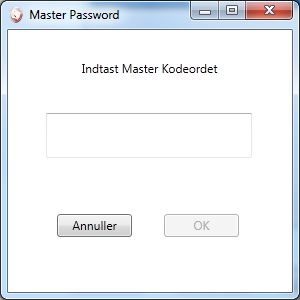
\includegraphics{CheckMasterPassword.png}
\end{center}
NOTICE: be aware that the system must always have at least four active machines to function. If this is not the case you are not able to start the election.
\item When the election has started you are presented with this page: \\
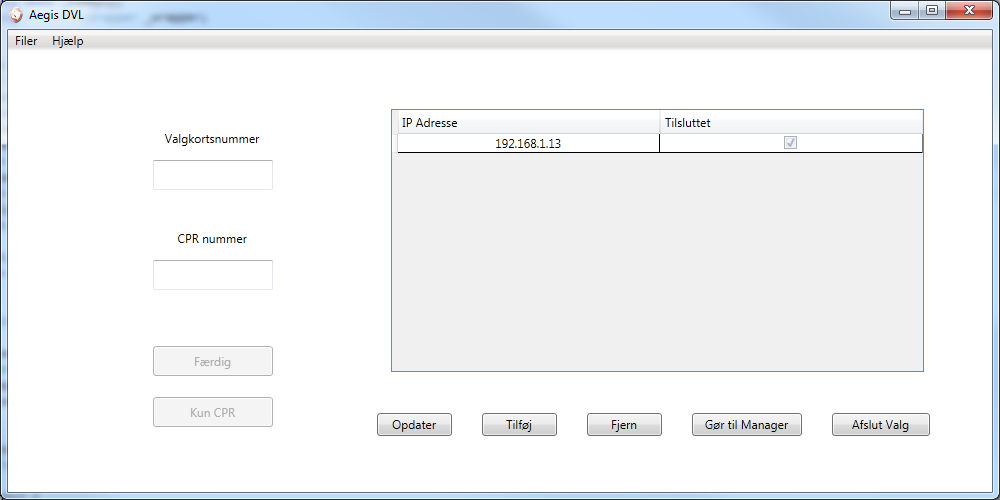
\includegraphics[width=\textwidth]{ManagerOverview.png}
This page is a combination of the previous page and the voting page from the station. The right side of the page functions exactly like the previous screen and the right side screen gives you the opportunity to mark voters with voter number and CPR number or just the CPR number provided you know the master password.
\item The only difference between the right side of the screen and the previous window is that the ''Start Valg'' has been replaced by ''Afslut Valg'' which lets you end the election provided you know the master password. When this is pressed the election ends, the station machines closes their applications and you are presented with this page: \\
\begin{center}
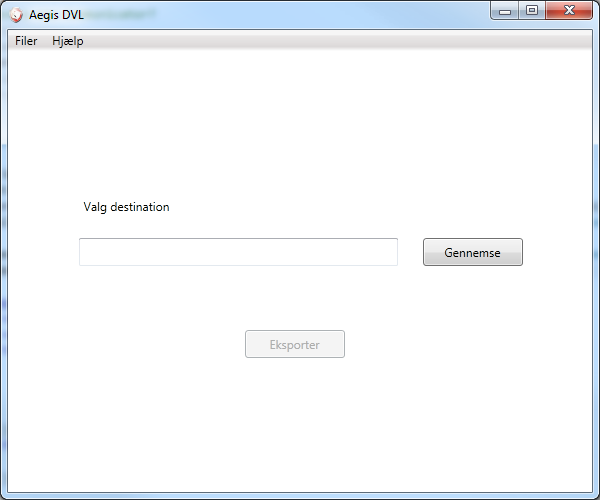
\includegraphics[width=100mm]{EndedElection.png}
\end{center}
\item Here you can export the voter data to a destination of your choice.
\end{enumerate}

\subsection*{Other}
At any time in the program you can choose "Marker v\ae lger", "Eksporter Data" or "Afslut" from the "Filer" menu or "Bruger manual" from the "Hj\ae lp" menu. \\
\begin{center}
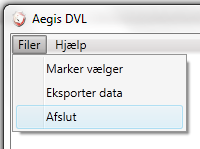
\includegraphics{FileMenu.png}
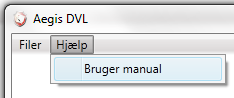
\includegraphics{HelpMenu.png}
\end{center}

\begin{itemize}
\item "Marker v\ae lger" opens this dialog: \\
\begin{center}
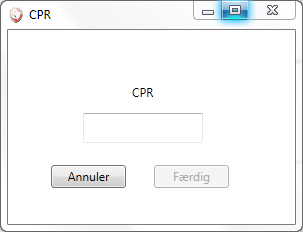
\includegraphics{BallotCPR.png}
\end{center}
Here you can mark a voter with only their CPR number, provided you know the master password. After you have entered the CPR number you are asked to enter the master password in this window: \\
\begin{center}
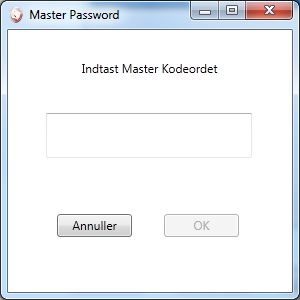
\includegraphics{CheckMasterPassword.png}
\end{center}
When this is done you can press ''OK'' and one of the following dialogues is shown: \\
\begin{center}
 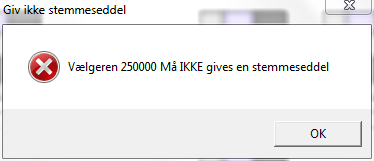
\includegraphics{BallotDenied.png}
\end{center}
This indicates that the voter is either not eligible to vote at this venue or that he has already been handed a ballot. \\
\begin{center}
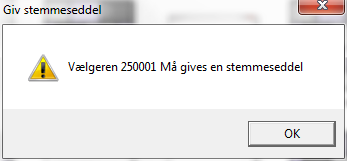
\includegraphics{BallotAccepted.png}
\end{center}
This indicates that the system has accepted the voter number and CPR number and that this voter can now be handed a ballot.

\item "Eksporter data" opens a dialog where you choose where to export the voter data. After you have chosen a destination, you are asked to enter the master password. When this is done successfully, the data is exported to the chosen location and the election continues.

\item ''Afslut'' asks you to enter the master password. If entered correctly, the application closes.

\item "Bruger manual" opens a PDF file containing this user manual.
\end{itemize}

If the manager machine should lose the connection to the network or lose power the remaining stations automatically elects one of the stations as the new manager and the user interface reflects it. \\

If the election should be a victim of an attack the detection triggers a shutdown of the entire election. This means this dialog appears on all machines: \\
\begin{center}

\includegraphics{ShutDownDialog.png}
\end{center}
When "OK" is pressed the application closes.

\section{UPPAAL}
\label{sec:uppaal}
\begin{center}
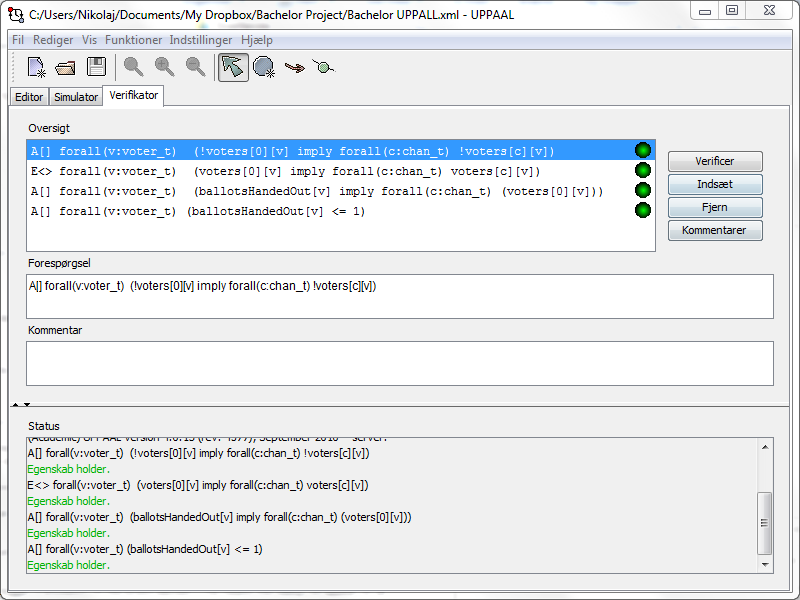
\includegraphics[width=\textwidth]{UPPAAL1.png}
\end{center}
\begin{center}
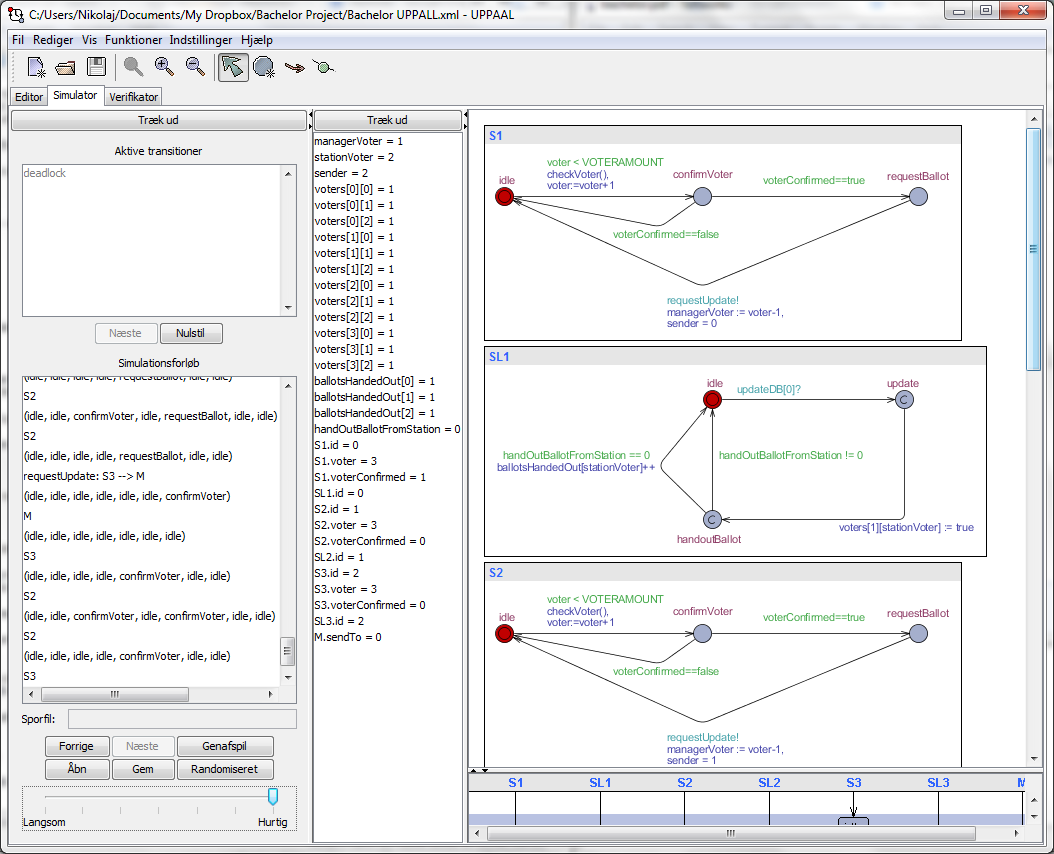
\includegraphics[width=\textwidth]{UPPAAL2.png}
\end{center}
\begin{center}
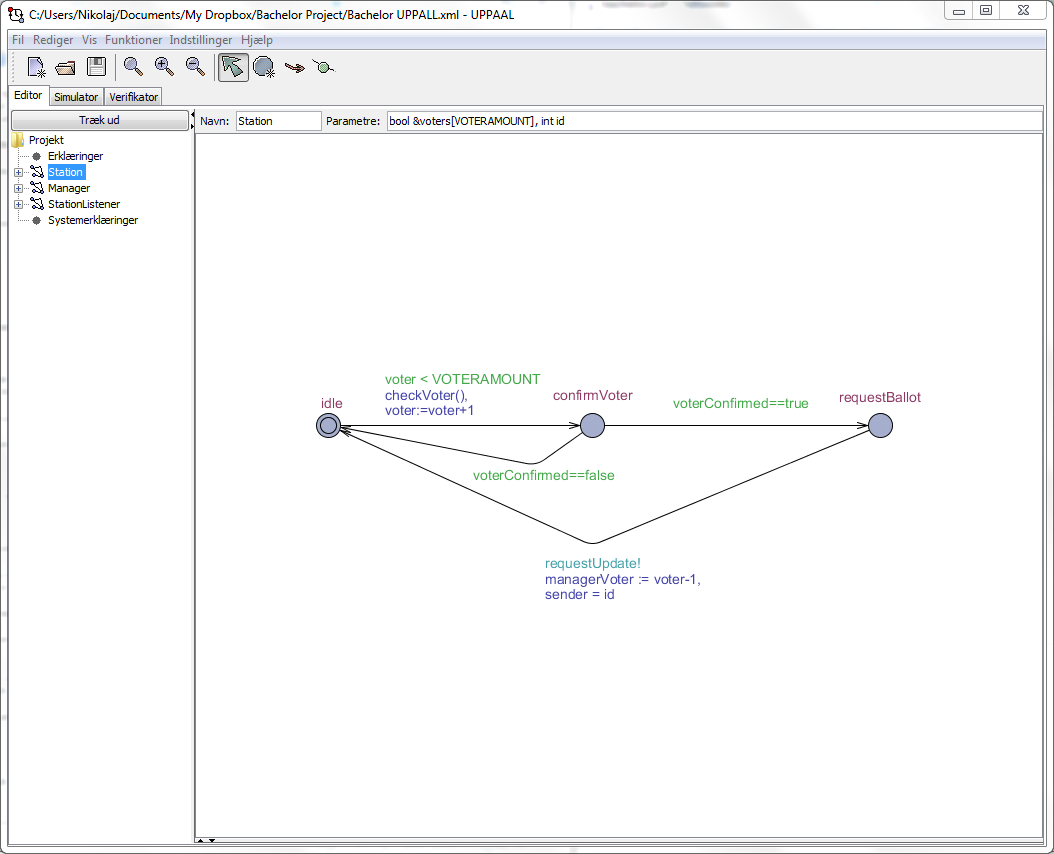
\includegraphics[width=\textwidth]{UPPAAL3.png}
\end{center}
\begin{center}
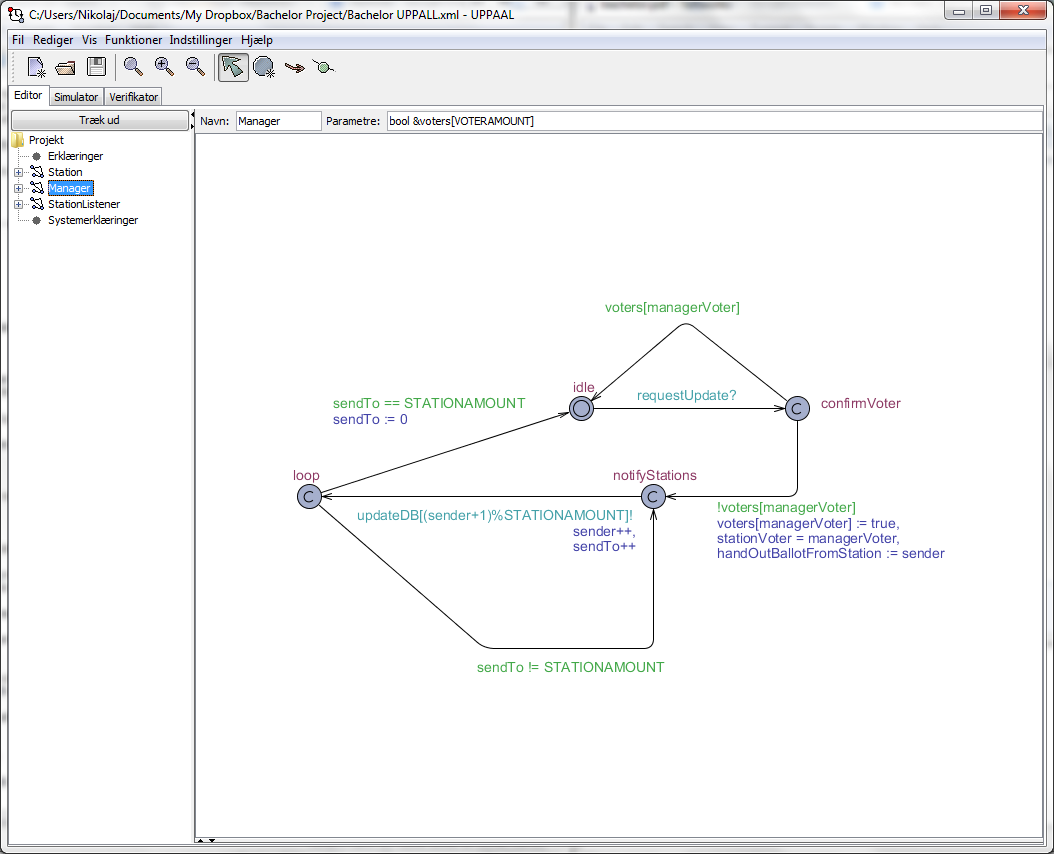
\includegraphics[width=\textwidth]{UPPAAL4.png}
\end{center}
\begin{center}
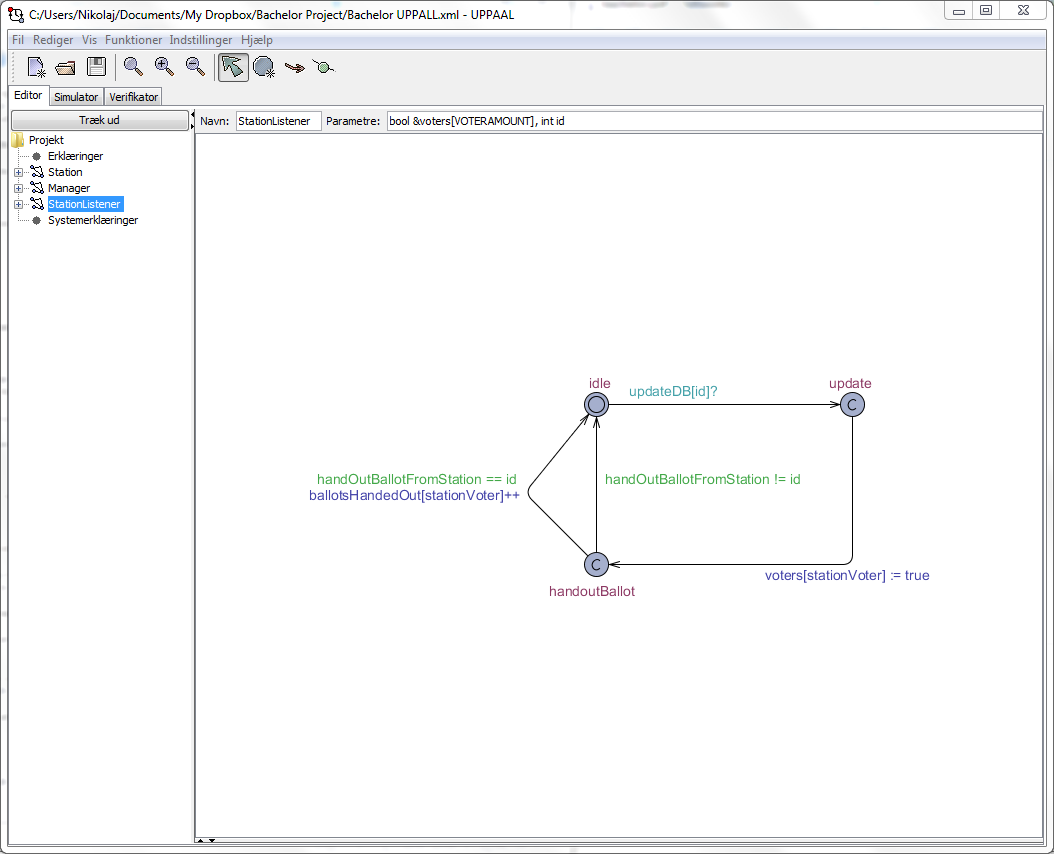
\includegraphics[width=\textwidth]{UPPAAL5.png}
\end{center}
\begin{center}
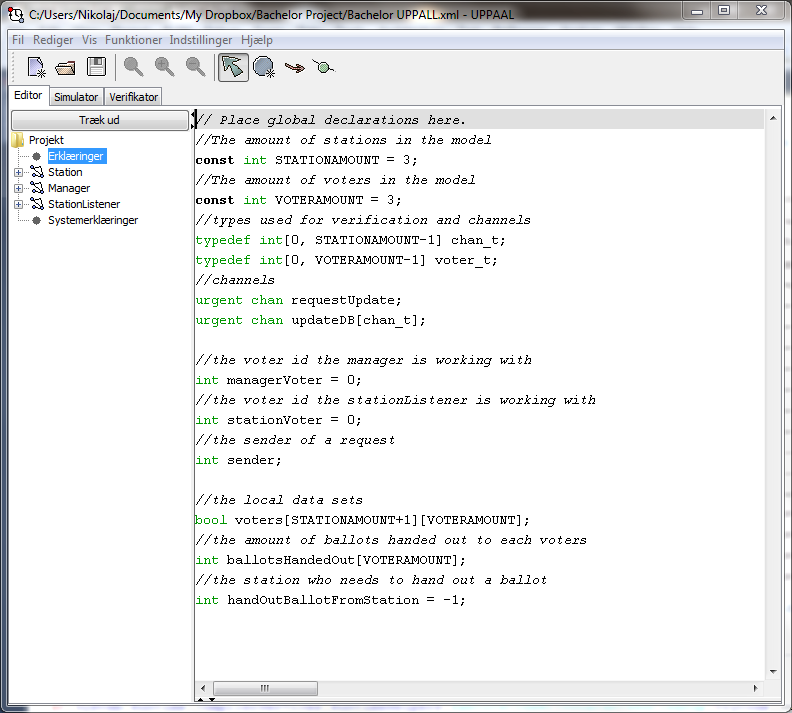
\includegraphics[width=\textwidth]{UPPAAL6.png}
\end{center}
\begin{center}
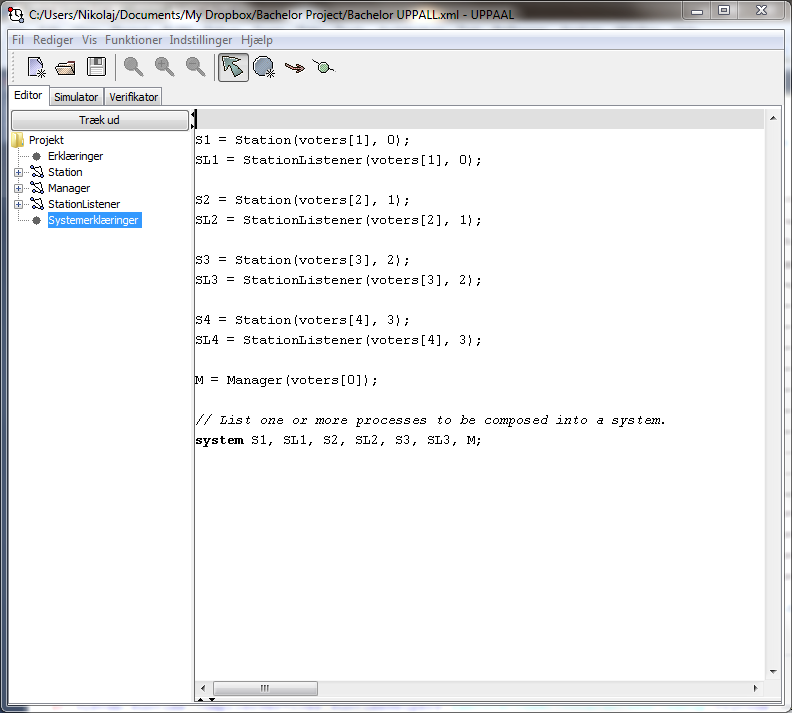
\includegraphics[width=\textwidth]{UPPAAL7.png}
\end{center}
\begin{center}
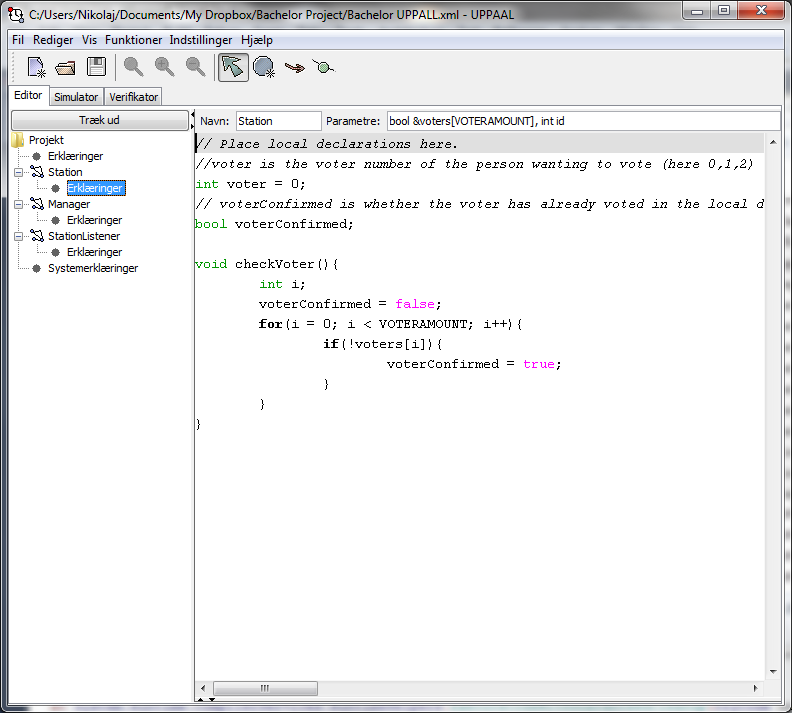
\includegraphics[width=\textwidth]{UPPAAL8.png}
\end{center}
\begin{center}
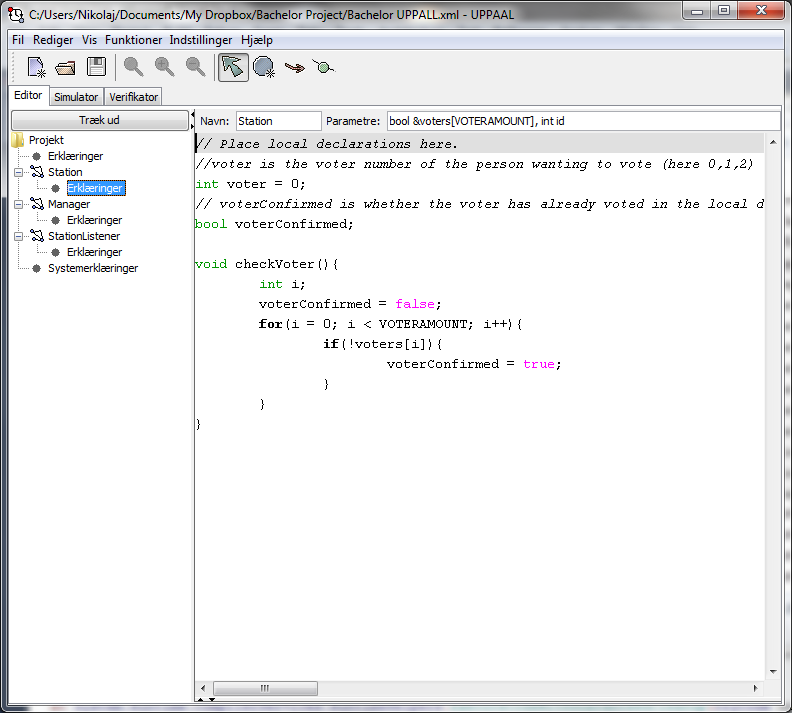
\includegraphics[width=\textwidth]{UPPAAL8.png}
\end{center}

\clearpage

\section{Attack trees}
Attack trees as described by Schneier in the notation described by Moore et al. with the addition of using $<$Attack pattern name$>$ to indicate the use of attack patterns in the attack tree. This should make the attacks trees less cluttered and make them easier to investigate. When the notation is used in an attack tree the attack pattern can be substituted in for the identifier.
We have also added a parentheses at the end of each action indication the cost of the action in Danish kroner, the number of people required to carry out the action, the technical skill needed to carry out the attack (high, medium or low) and the likelihood of the attack rated from 1 to 5, where 1 is very unlikely and 5 is very likely.\\

\noindent Example:
\begin{verbatim}
2. Manipulate person(s) responsible for partitioning to manipulate the data
   <Manipulate person(s)>
	
is equivalent to

2. Manipulate person(s) responsible for partitioning to manipulate the data
     OR     1. Bribe them (20.000/1/low/3)
            2. Force them (0/1/low/4)
            3. Threaten them (0/1/low/4)
\end{verbatim}

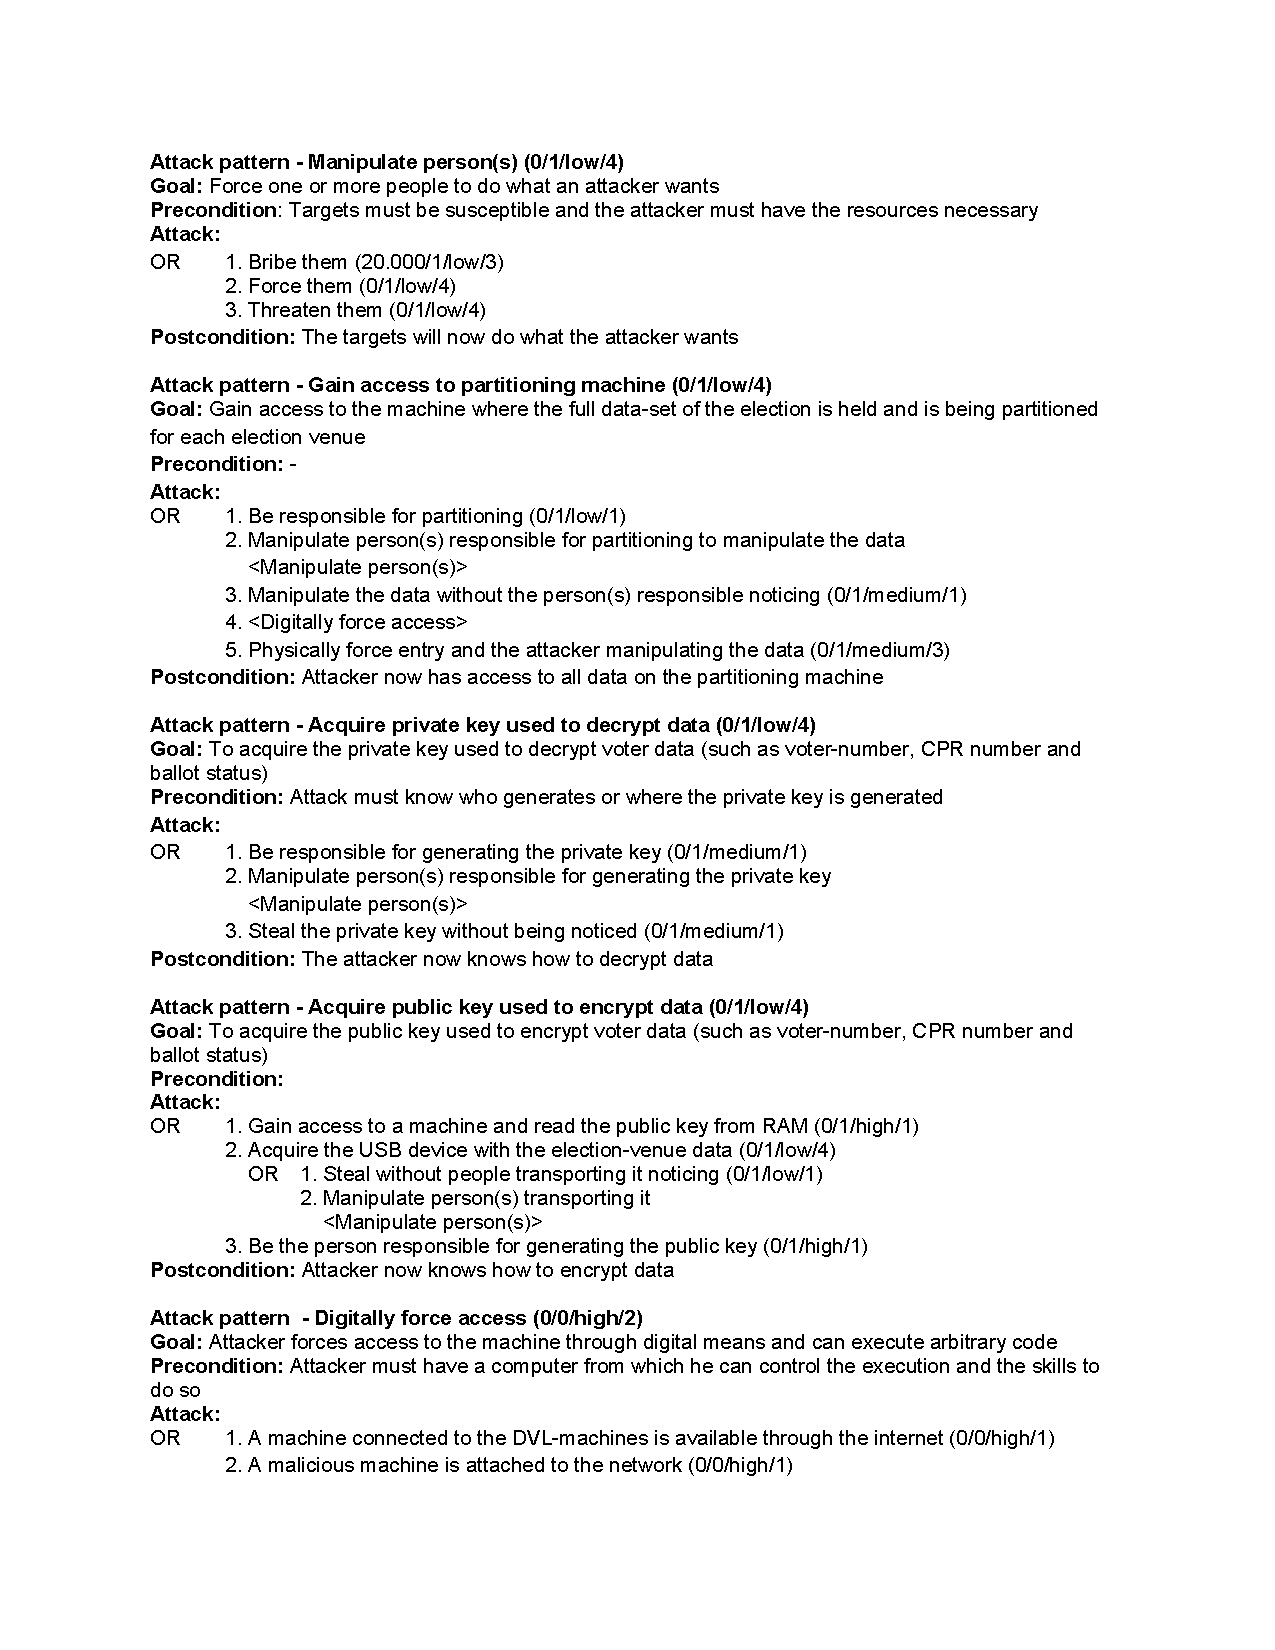
\includepdf[pages=-]{AttackTrees.pdf}

\label{sec:atrees}

\section{Revision history}
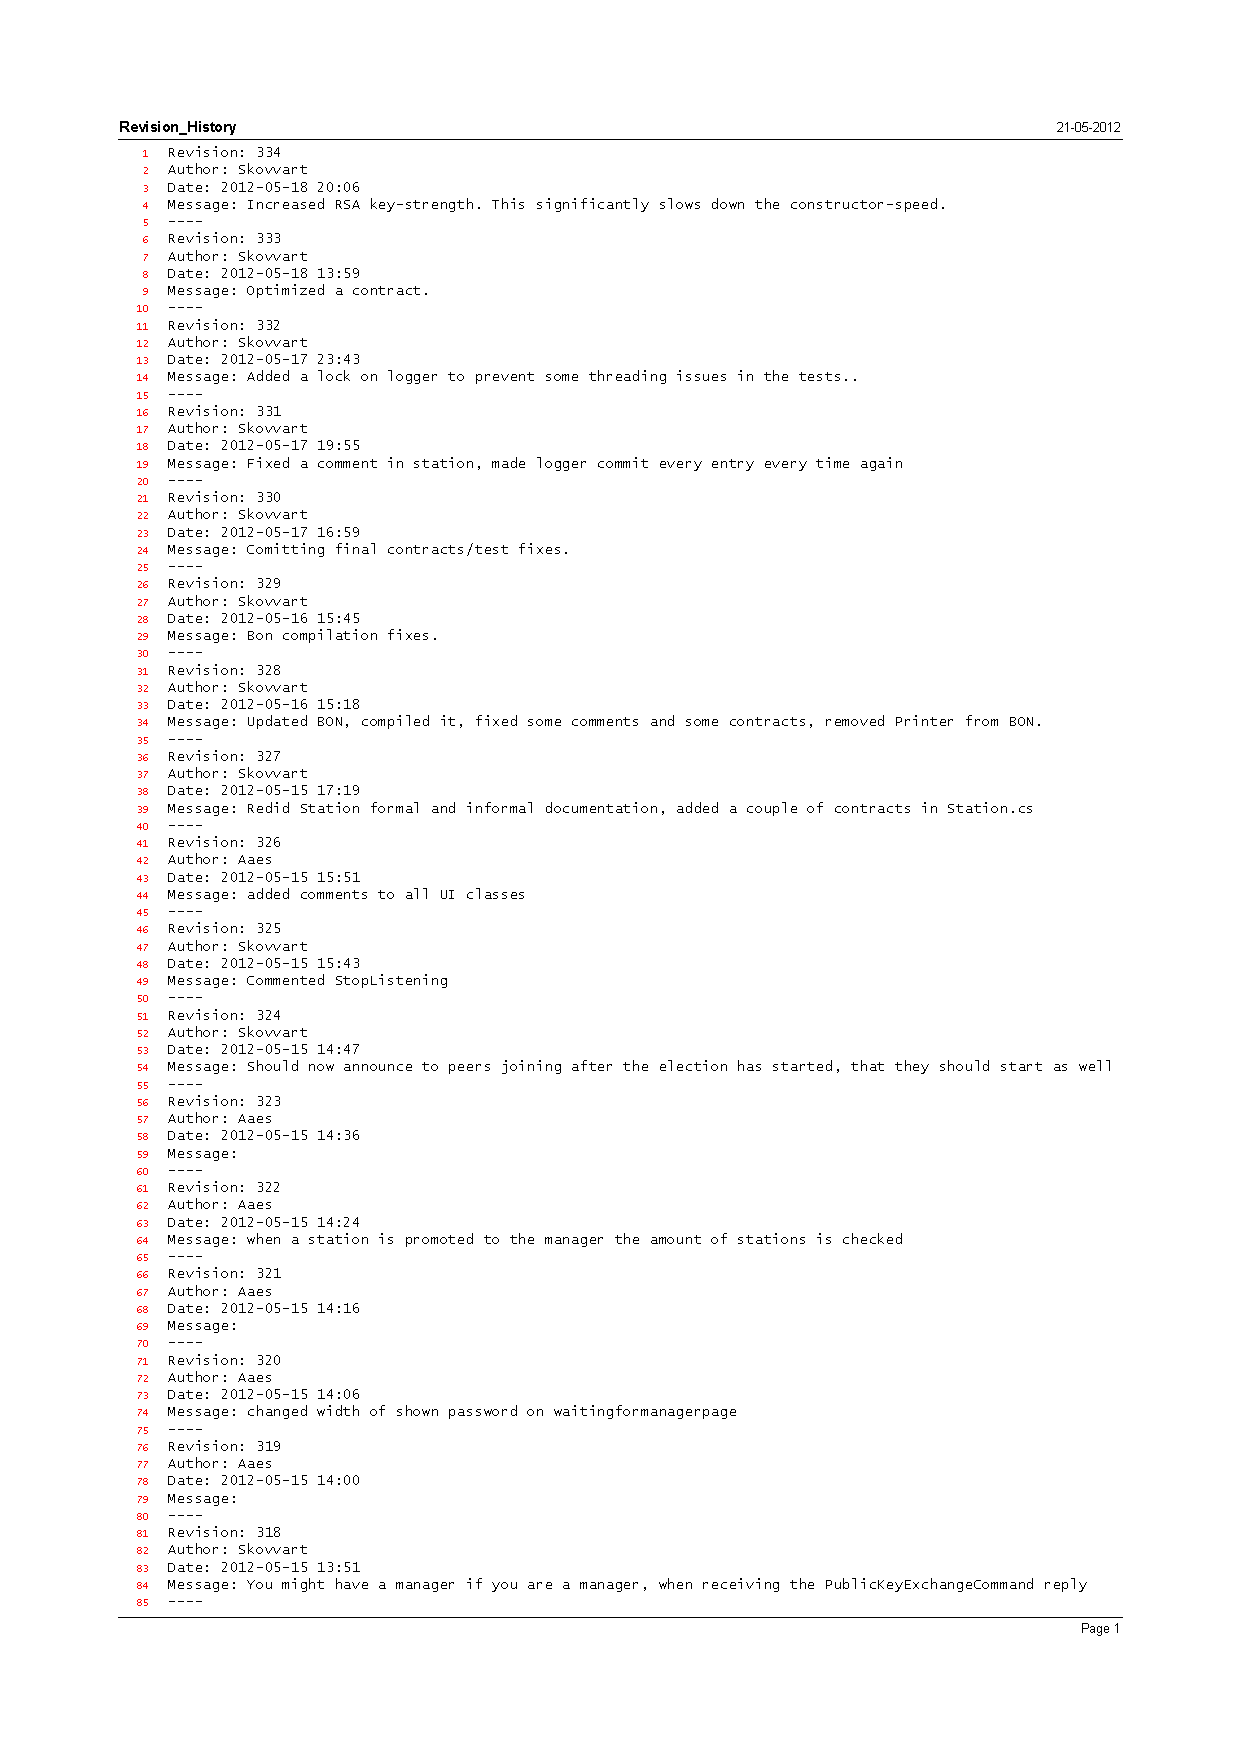
\includepdf[pages=-]{Revision_History.pdf}

\section{BON}
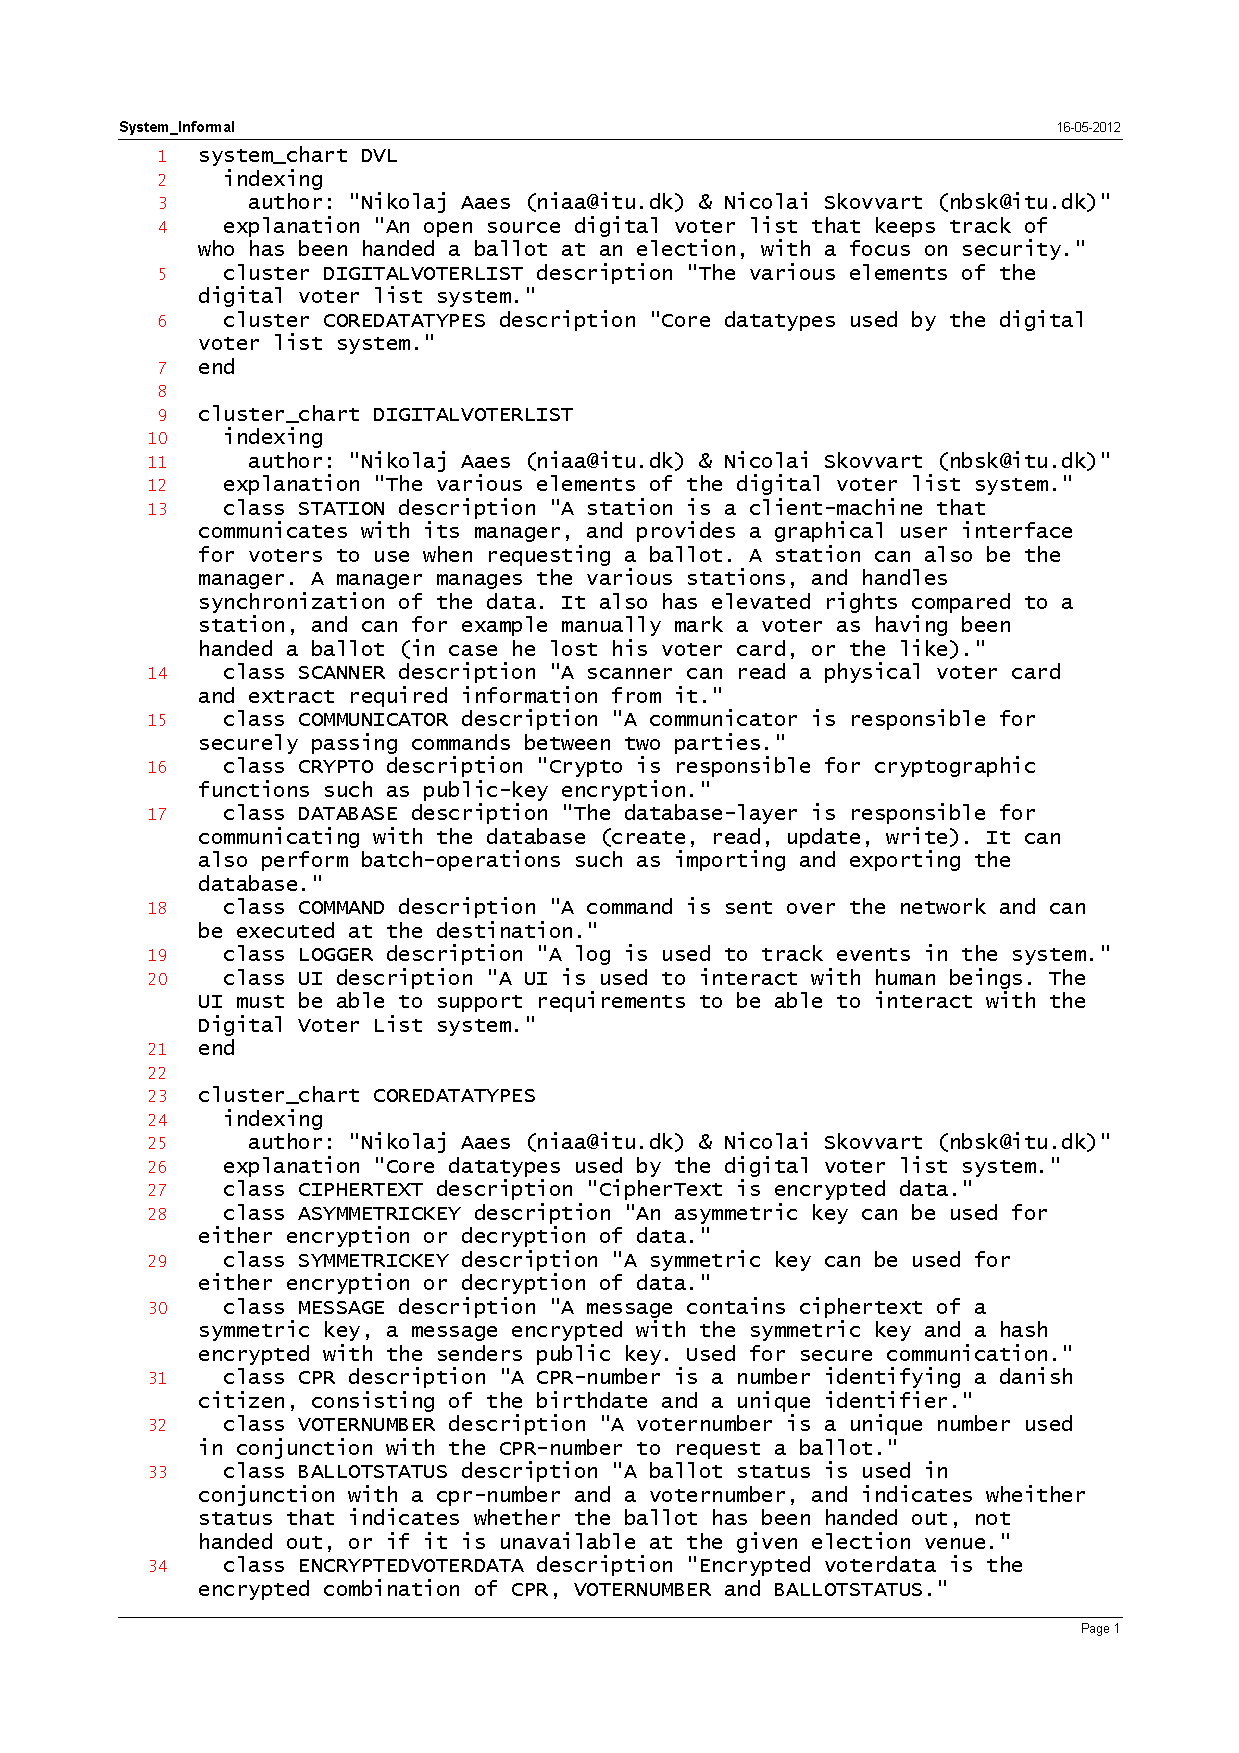
\includepdf[pages=-]{BONPDF/System_Informal.pdf}
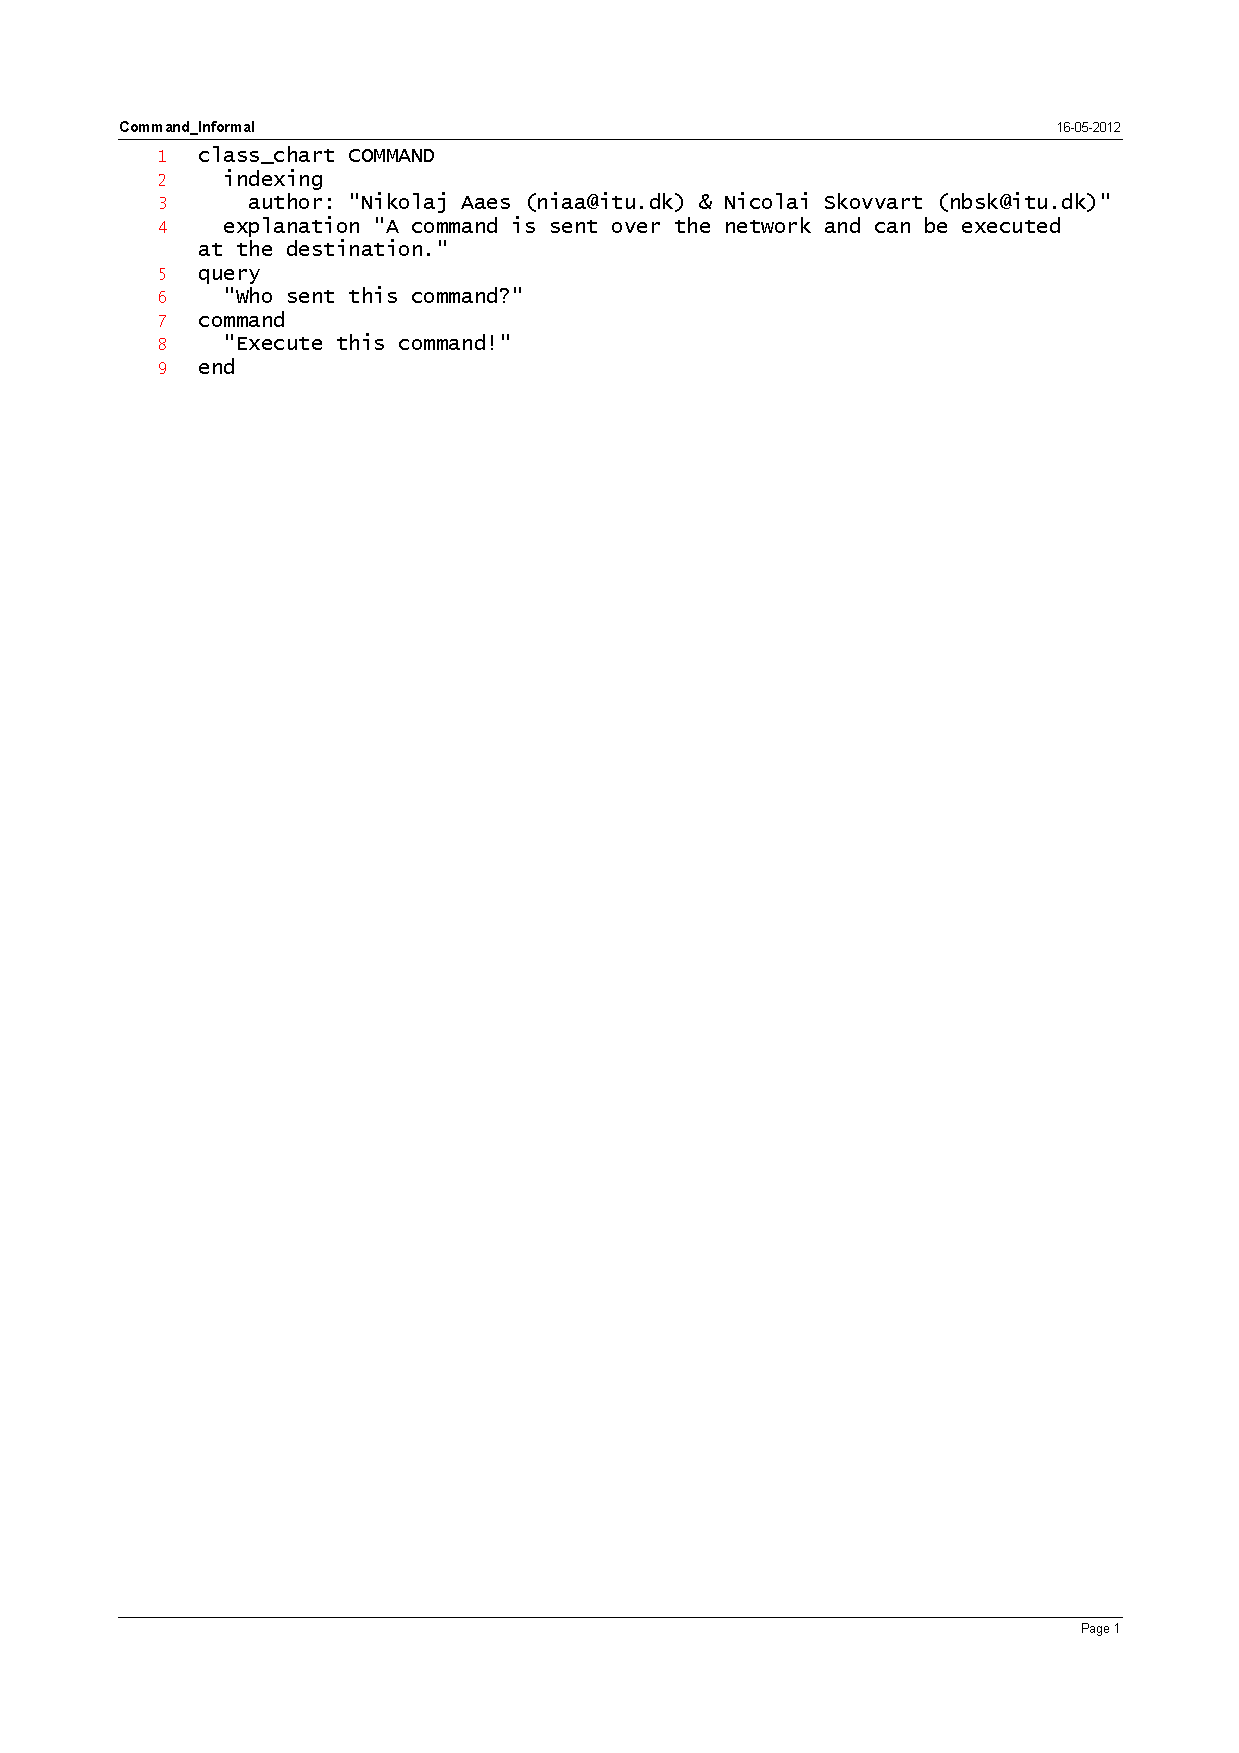
\includepdf[pages=-]{BONPDF/Command_Informal.pdf}
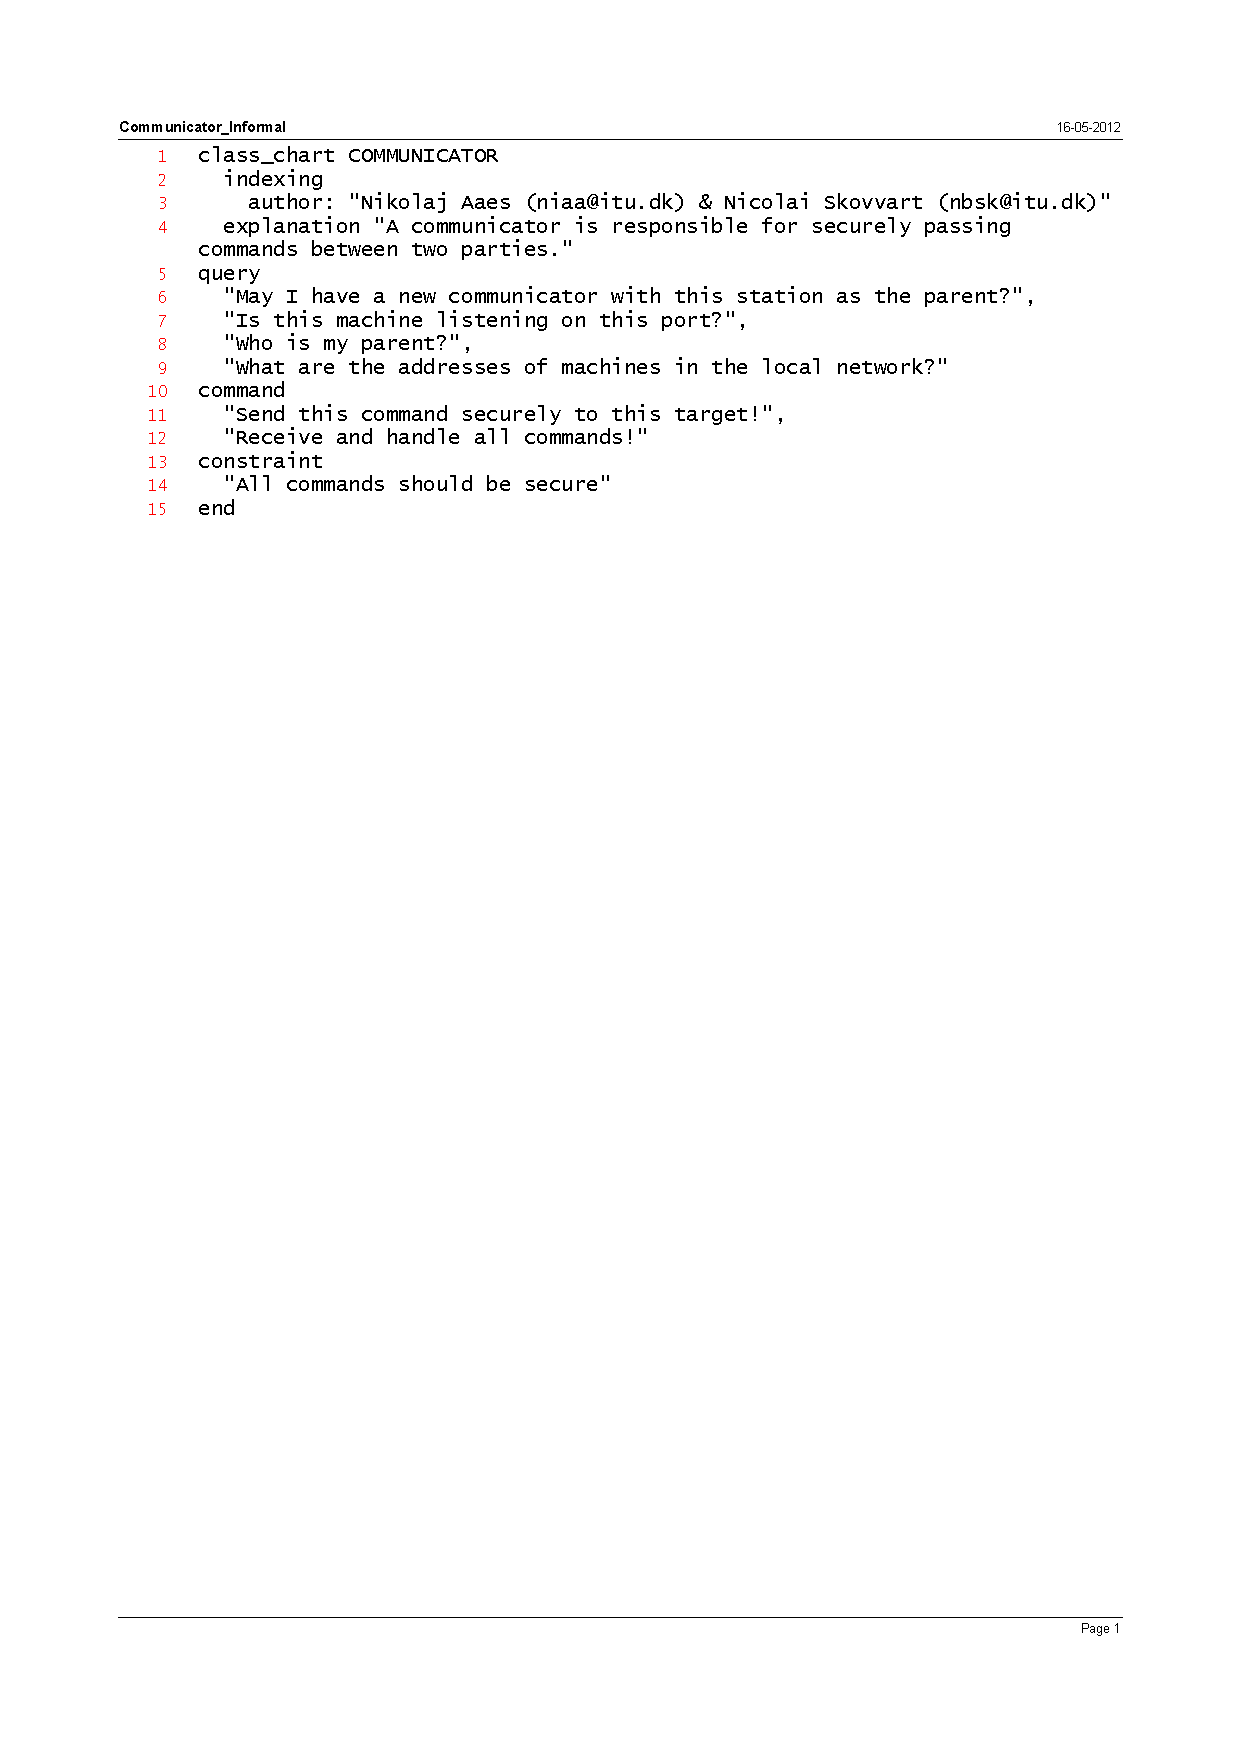
\includepdf[pages=-]{BONPDF/Communicator_Informal.pdf}
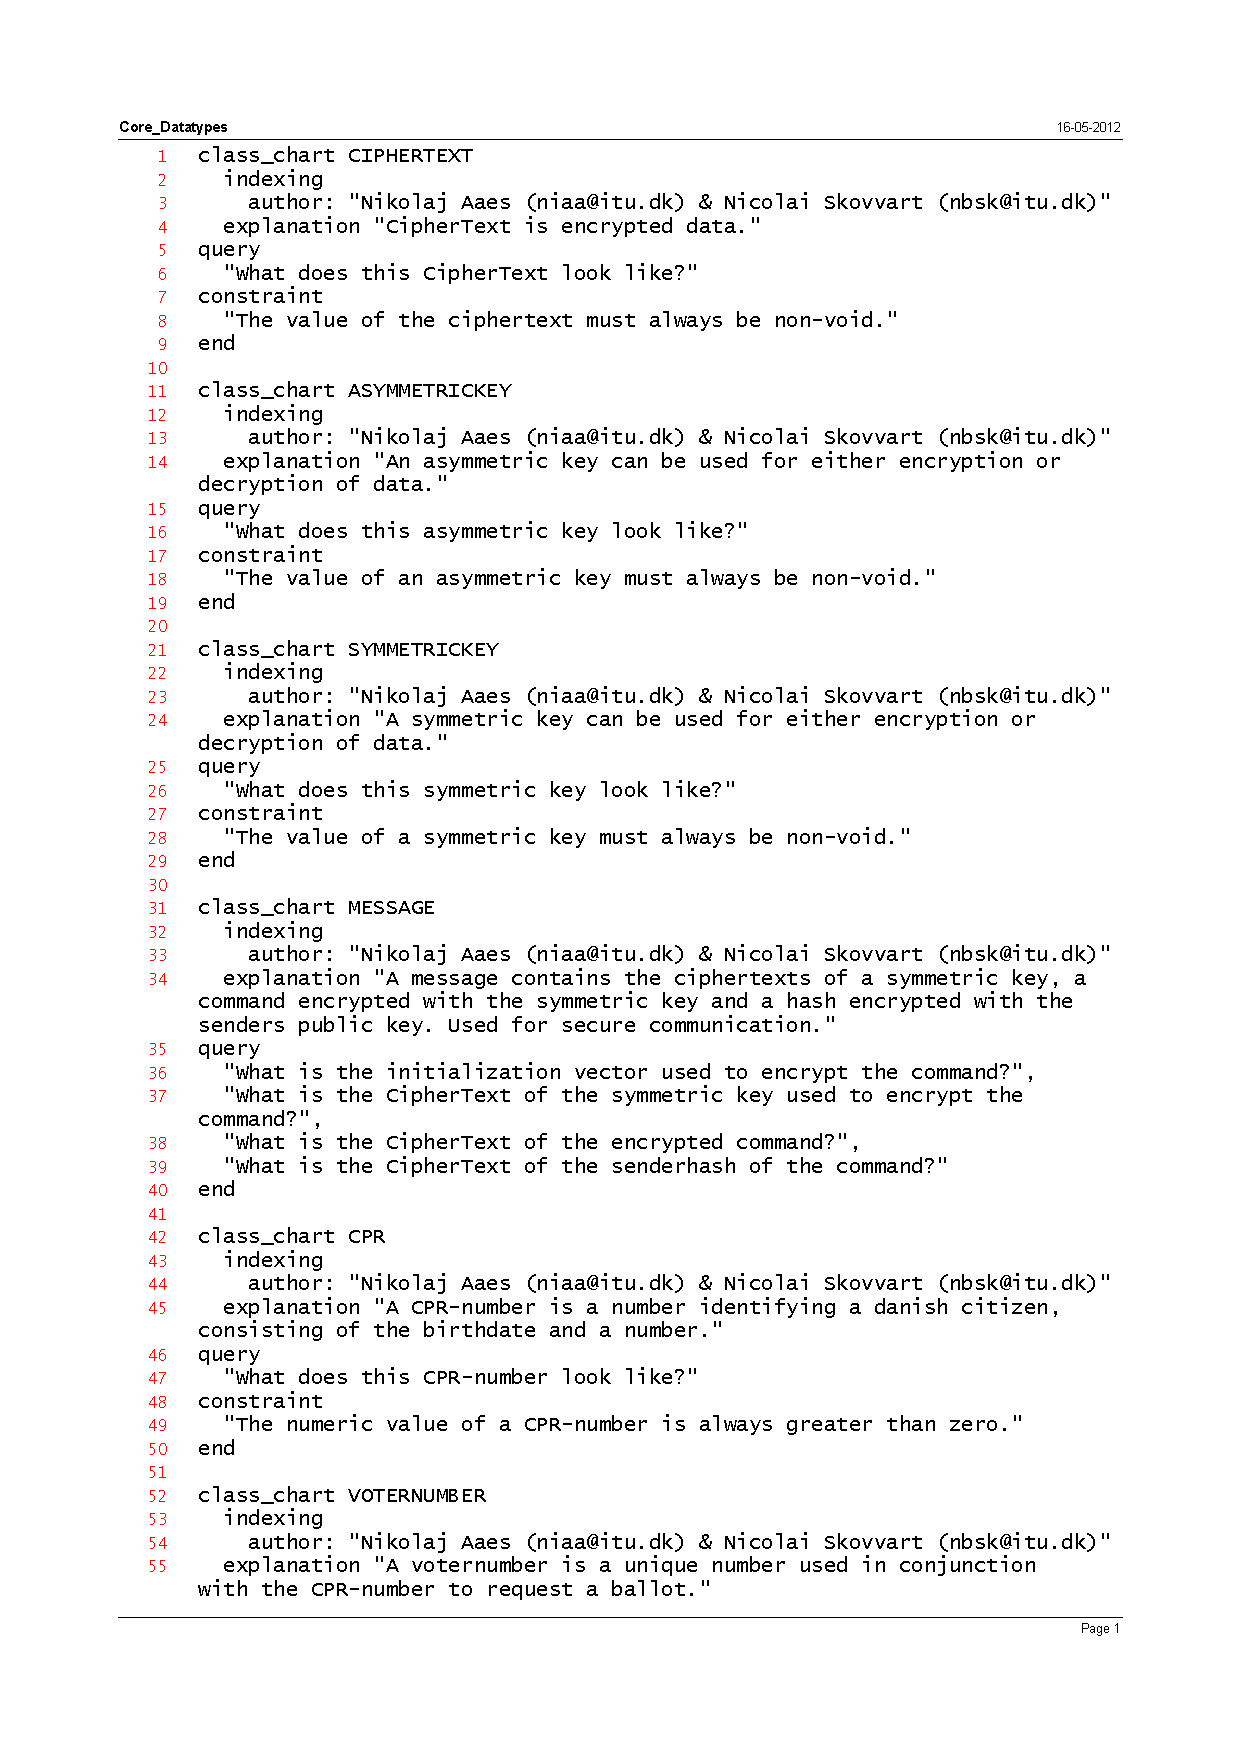
\includepdf[pages=-]{BONPDF/Core_Datatypes_Informal.pdf}
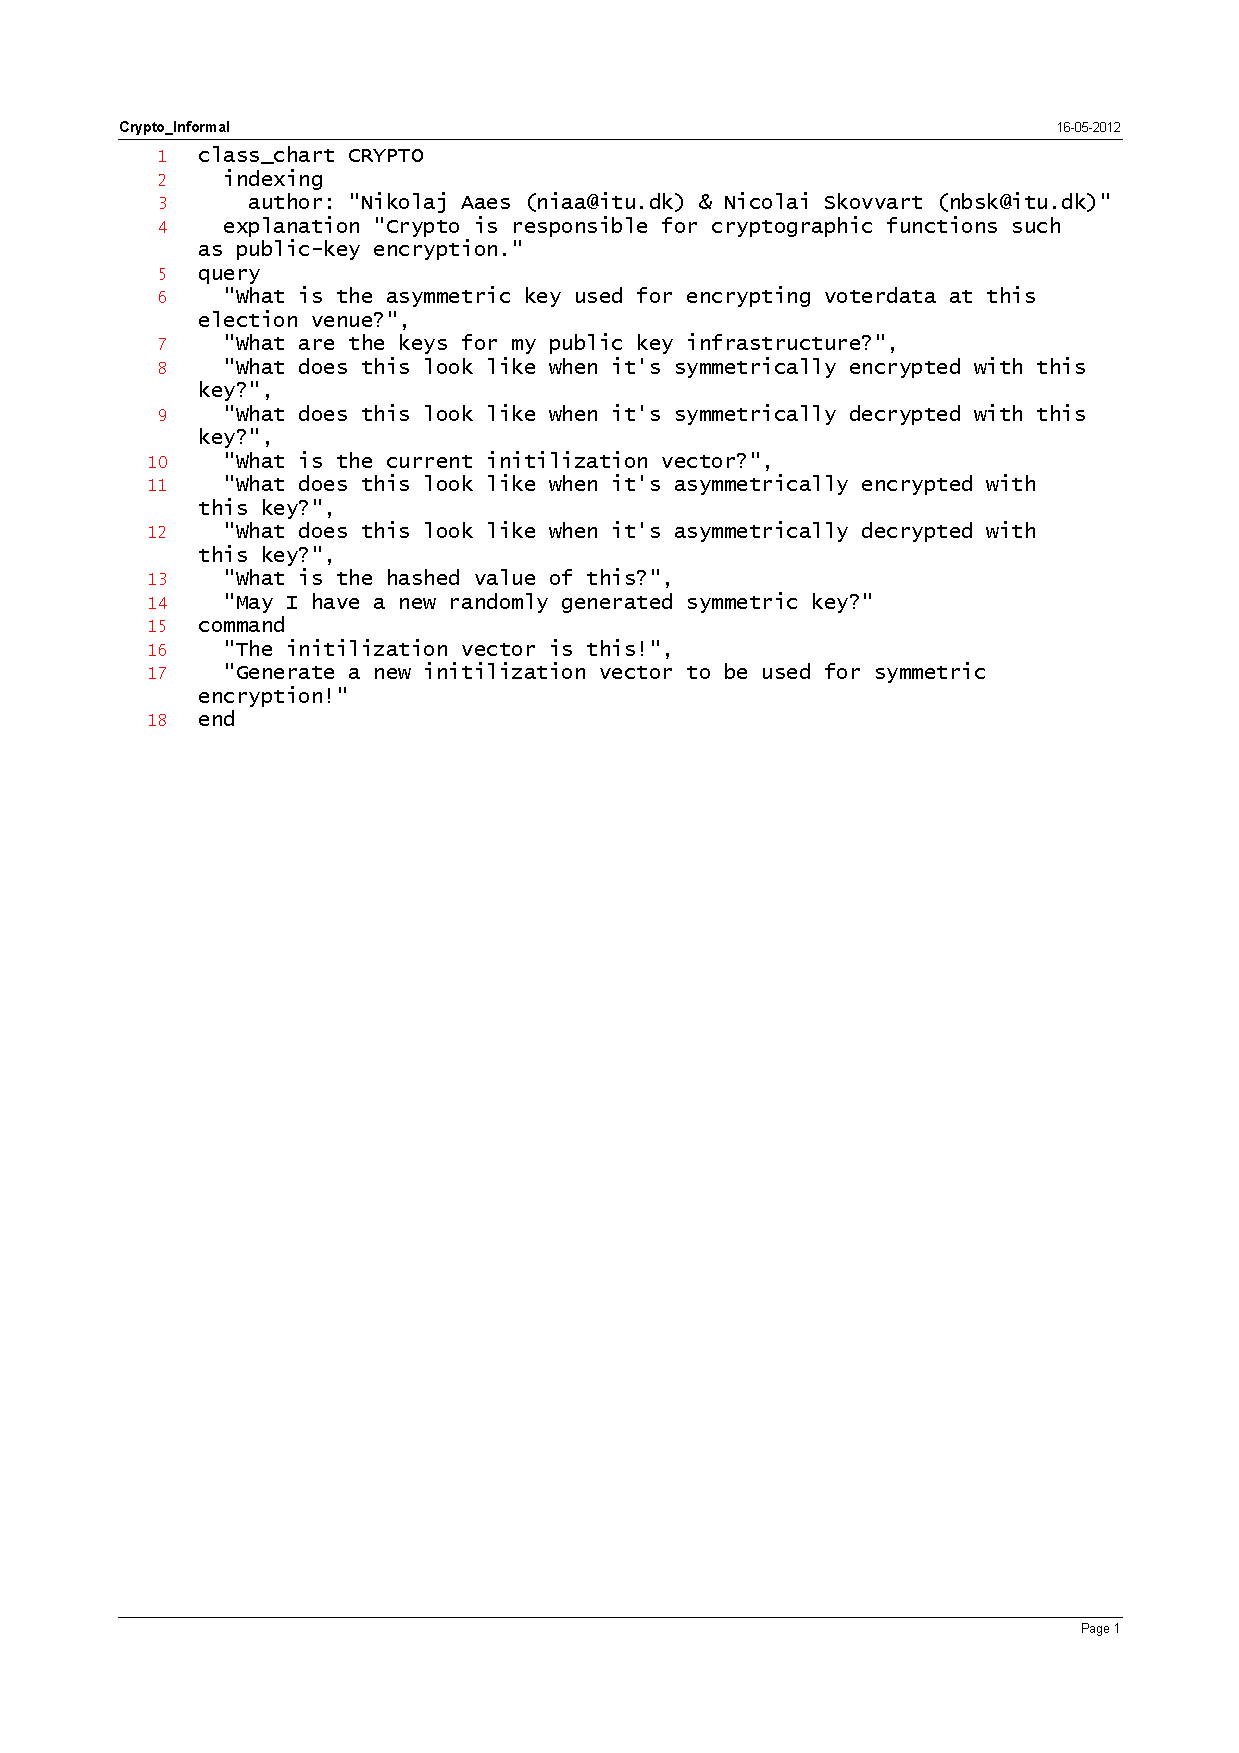
\includepdf[pages=-]{BONPDF/Crypto_Informal.pdf}
\includepdf[pages=-]{BONPDF/Database_Informal.pdf}
\includepdf[pages=-]{BONPDF/Logger_Informal.pdf}
\includepdf[pages=-]{BONPDF/Scanner_Informal.pdf}
\includepdf[pages=-]{BONPDF/Station_Informal.pdf}
\includepdf[pages=-]{BONPDF/UI_Informal.pdf}


\includepdf[pages=-]{BONPDF/Command_Formal.pdf}
\includepdf[pages=-]{BONPDF/Communicator_Formal.pdf}
\includepdf[pages=-]{BONPDF/Core_Datatypes_Formal.pdf}
\includepdf[pages=-]{BONPDF/Crypto_Formal.pdf}
\includepdf[pages=-]{BONPDF/Database_Formal.pdf}
\includepdf[pages=-]{BONPDF/Logger_Formal.pdf}
\includepdf[pages=-]{BONPDF/Scanner_Formal.pdf}
\includepdf[pages=-]{BONPDF/Station_Formal.pdf}
\includepdf[pages=-]{BONPDF/UI_Formal.pdf}

\end{document}